\chapter{Requisitos do Sistema}

\section{Análise e Levantamento dos Requisitos}
A aplicação a desenvolver deverá suportar o registo das despesas e a gestão do seu pagamento por parte de moradores registados.

\subsection{Criação do grupo com os elementos da casa/apartamento}

\begin{itemize}
	

\item{Cada morador deve efetuar um registo fornecendo o seu nome, e-mail, número de telemóvel e data de nascimento.}

\item{O morador assim como o utilizador necessitam de efetuar login na aplicação}

\item{O utilizador que convidar os restantes será considerado adminstrador do sistema.} 

\end{itemize}

\subsection{Gestão das contas}

\begin{itemize}
	
\item{Após o registo será associada uma conta corrente a cada utilizador.}

\item{Cada conta corrente permitirá a gestão do saldo corrente (estão incluidas dívidas) de cada morador.}

\item{O morador deverá efetuar um pagamento.}
 
\item{Cada pagamento será creditado na conta corrente do morador.}

\item{Cada pagamento efetuado não pode ultrapassar o valor da fatura}
 
 \item{O pagamento pode ser igual ou superior à quantia necessária para pagar as despesas em causa.}
 
 
\item{Existirá um saldo global da casa, este que é o somatório de todas as contas correntes dos moradores}
 
 \item{O saldo global é administrado por um Adminstrador}
 
\item{Existem dois tipos de despesas distintos: a despesa recorrente referente a despesas mensais como a água, luz, renda, etc; a despesa extra referente a por exemplo arranjos de material na casa}
 
\item{Cada morador deverá pagar uma fração relativa à despesa}
 
\item{Cada despesa a pagar tem a si associado um tipo (i.e. água, luz, cadeiras, etc)}

\end{itemize}


\section{Base de dados }
A aplicação necessitará de uma implementação de uma base de dados para gerir os elementos que pertencem ao grupo assim como as despesas efetuadas pelos moradores. A modelação concetual consiste no processo de construção de um modelo de dados a partir de uma análise detalhada dos requisitos.  Este modelo é completamente independente de todas as considerações físicas, ou seja é independente dos detalhes de implementação. De seguida está aprsentado o esquema concetual relativo ao projeto.  


\begin{figure}[htb!]
	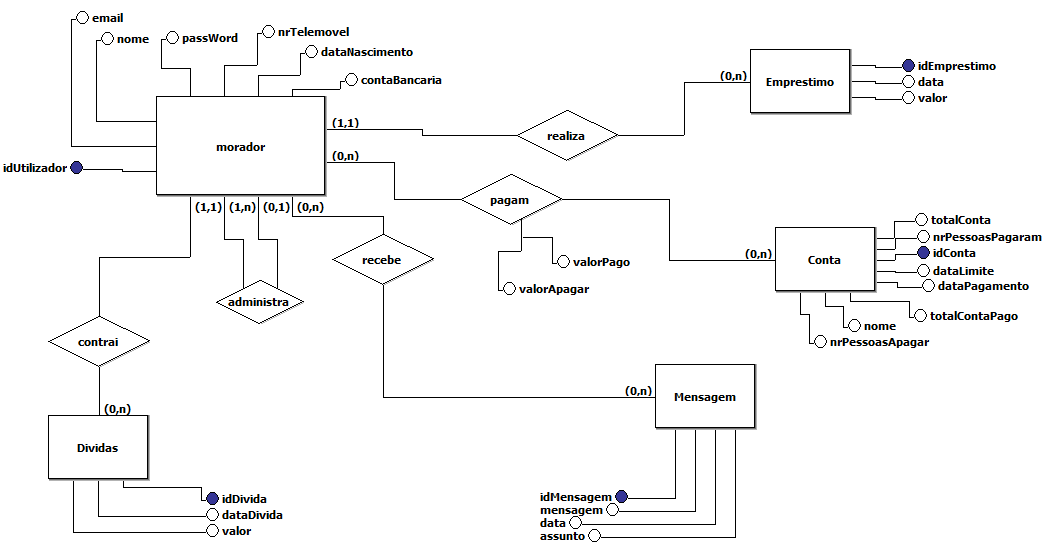
\includegraphics[scale=0.6]{imagens/bd/modeloconcetual}  
	\caption{Modelo Concetual}  
\end{figure}

\newpage

Terminada a modelação concetual, procedemos à fase de modelação lógica. Esta consiste na tradução do modelo concetual para o lógico capaz de representar os requisitos definidos, assim como a validação do mesmo. Este modelo está representado na figura abaixo: 

\begin{figure}[htb!]
	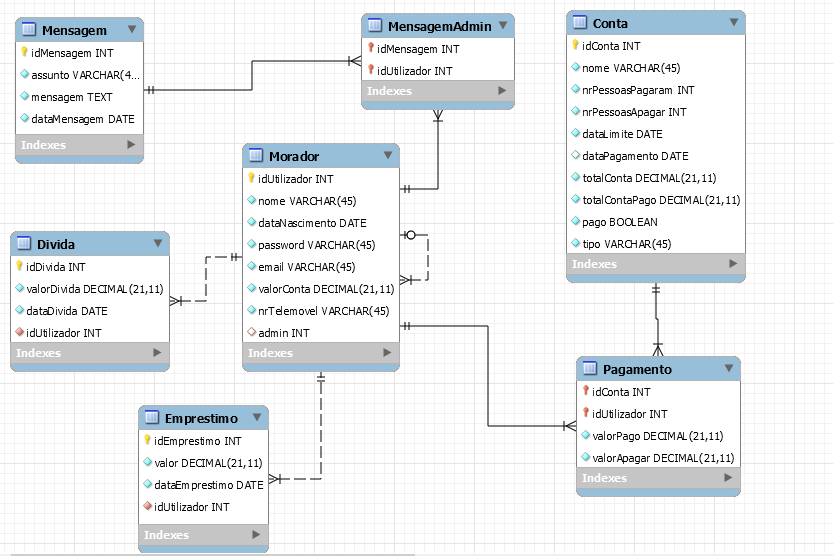
\includegraphics[scale=0.7]{imagens/bd/modelologico}  
	\caption{Modelo Lógico}  
\end{figure}

\newpage

Para a realização deste projeto, construímos uma base de dados relacional em \textit{MySQL} para armazenar toda a informação necessária para colocar o SGD \footnote{Sistema de Gestão de Despesas} a correr. Para o programa aceder a essa informação, foram classes \textit{DAO} \footnote{Data Acess Object} , que fornecem métodos de acesso à base de dados. Cada método visível para o exterior
destas classe solicita sempre uma conecção à base de Dados, este pedido é feito à classe \textit{Connector}, podendo este conetor estar configurado com Auto-Commit ou não dependendo do tipo de operações pretendidas.
São também definidos métodos auxiliares alguns \textit{Private} e outros \textit{Protected} que executam as queries à base de dados, contêm \textit{PreparedStatements} por questões de segurança contra SQL \textit{injection}. A criação destes métodos deve-se à tentativa de minimizar as conceções simultâneas à Base de Dados.


\begin{figure}[htb!]
	\centering
	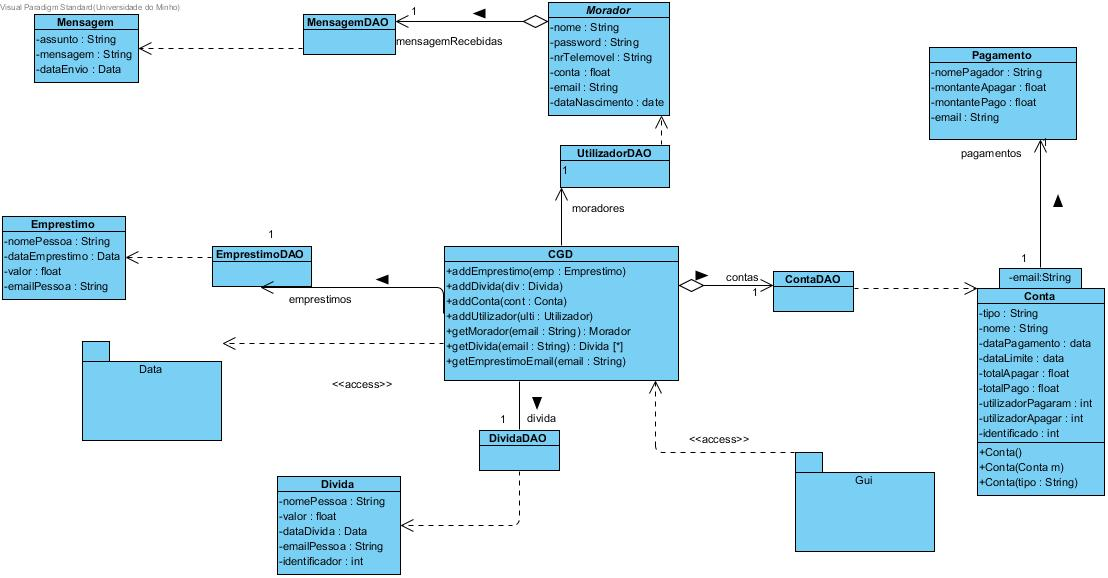
\includegraphics[scale=0.2]{imagens/diagramaClasses/DiagramaClasseDAO}  
	\caption{Diagrama de Classes DAO  }  
\end{figure}


\chapter{Arquitetura da Aplicação}

\section{Modelo de Dominio }
Todo e qualquer projeto possui um domínio específico. O modelo de domínio deve capturar os seguintes pontos: as entidades, os relacionamentos entre as entidades e o vocabulário de domínio do problema. Para além disso também deve ser uma visão estática do problema onde é possível representar as regras de negócio invariantes no tempo. Ou seja, o modelo de domínio é a base para a análise de requisitos.

No que diz respeito à aplicação, como é dito na introdução, queremos desenvolver uma aplicação capaz de suportar o registo das despesas e a gestão do seu pagamento por parte dos moradores registados.


\begin{figure}[htb!]
	\includegraphics[scale=0.4]{imagens/mD/"ModeloDominio"}  
	\caption{Modelo Dominio}  
\end{figure}

O morador necessita de fornecer o nome, e-mail, número de telemovel e data de nascimento, para se registar. 

Para efetuar login será necessário inserir o e-mail e a palavra passe. 

Como se pode observar na figura o morador efetua pagamento relativo a despesa recorrente ou extra, assim como paga uma fração da despesa, essa fração é relativa a um tipo de despesa. 


O administrador administra o saldo global da casa/apartamento. 


\newpage

\section{Diagrama de Classes}
A metodologia de implementação das boas práticas do UML no desenvolvimento de qualquer
projecto, especialmente em projectos de media e pequena escala, para possíveis implementações de ideias da camada de negócio e de esquemas conceptuais, que podem ser validados e discutidos pelo grupo de desenvolvimento e analisados sem que seja necessário perder tempo com testes e builds.
No caso especifico do diagrama de classes aquilo que concluímos é que permite de uma forma simples e transparente partilhar e discutir como irá ser, ou pelos menos como se pretende que seja, os esquemas
conceptuais do modelo de domínio e esqueleto do nossa implementação, ou seja, das estrutura básica das classes. O modelo abaixo apresentado é portanto uma tradução daquilo que pretendíamos com o
modelo de domínio, mas nesse caso, com maior detalhe técnico relativos à linguagem de programação escolhida, i.e. o Java. Temos portanto o seguinte diagrama de classes:

\begin{figure}[htb!]
	\centering
	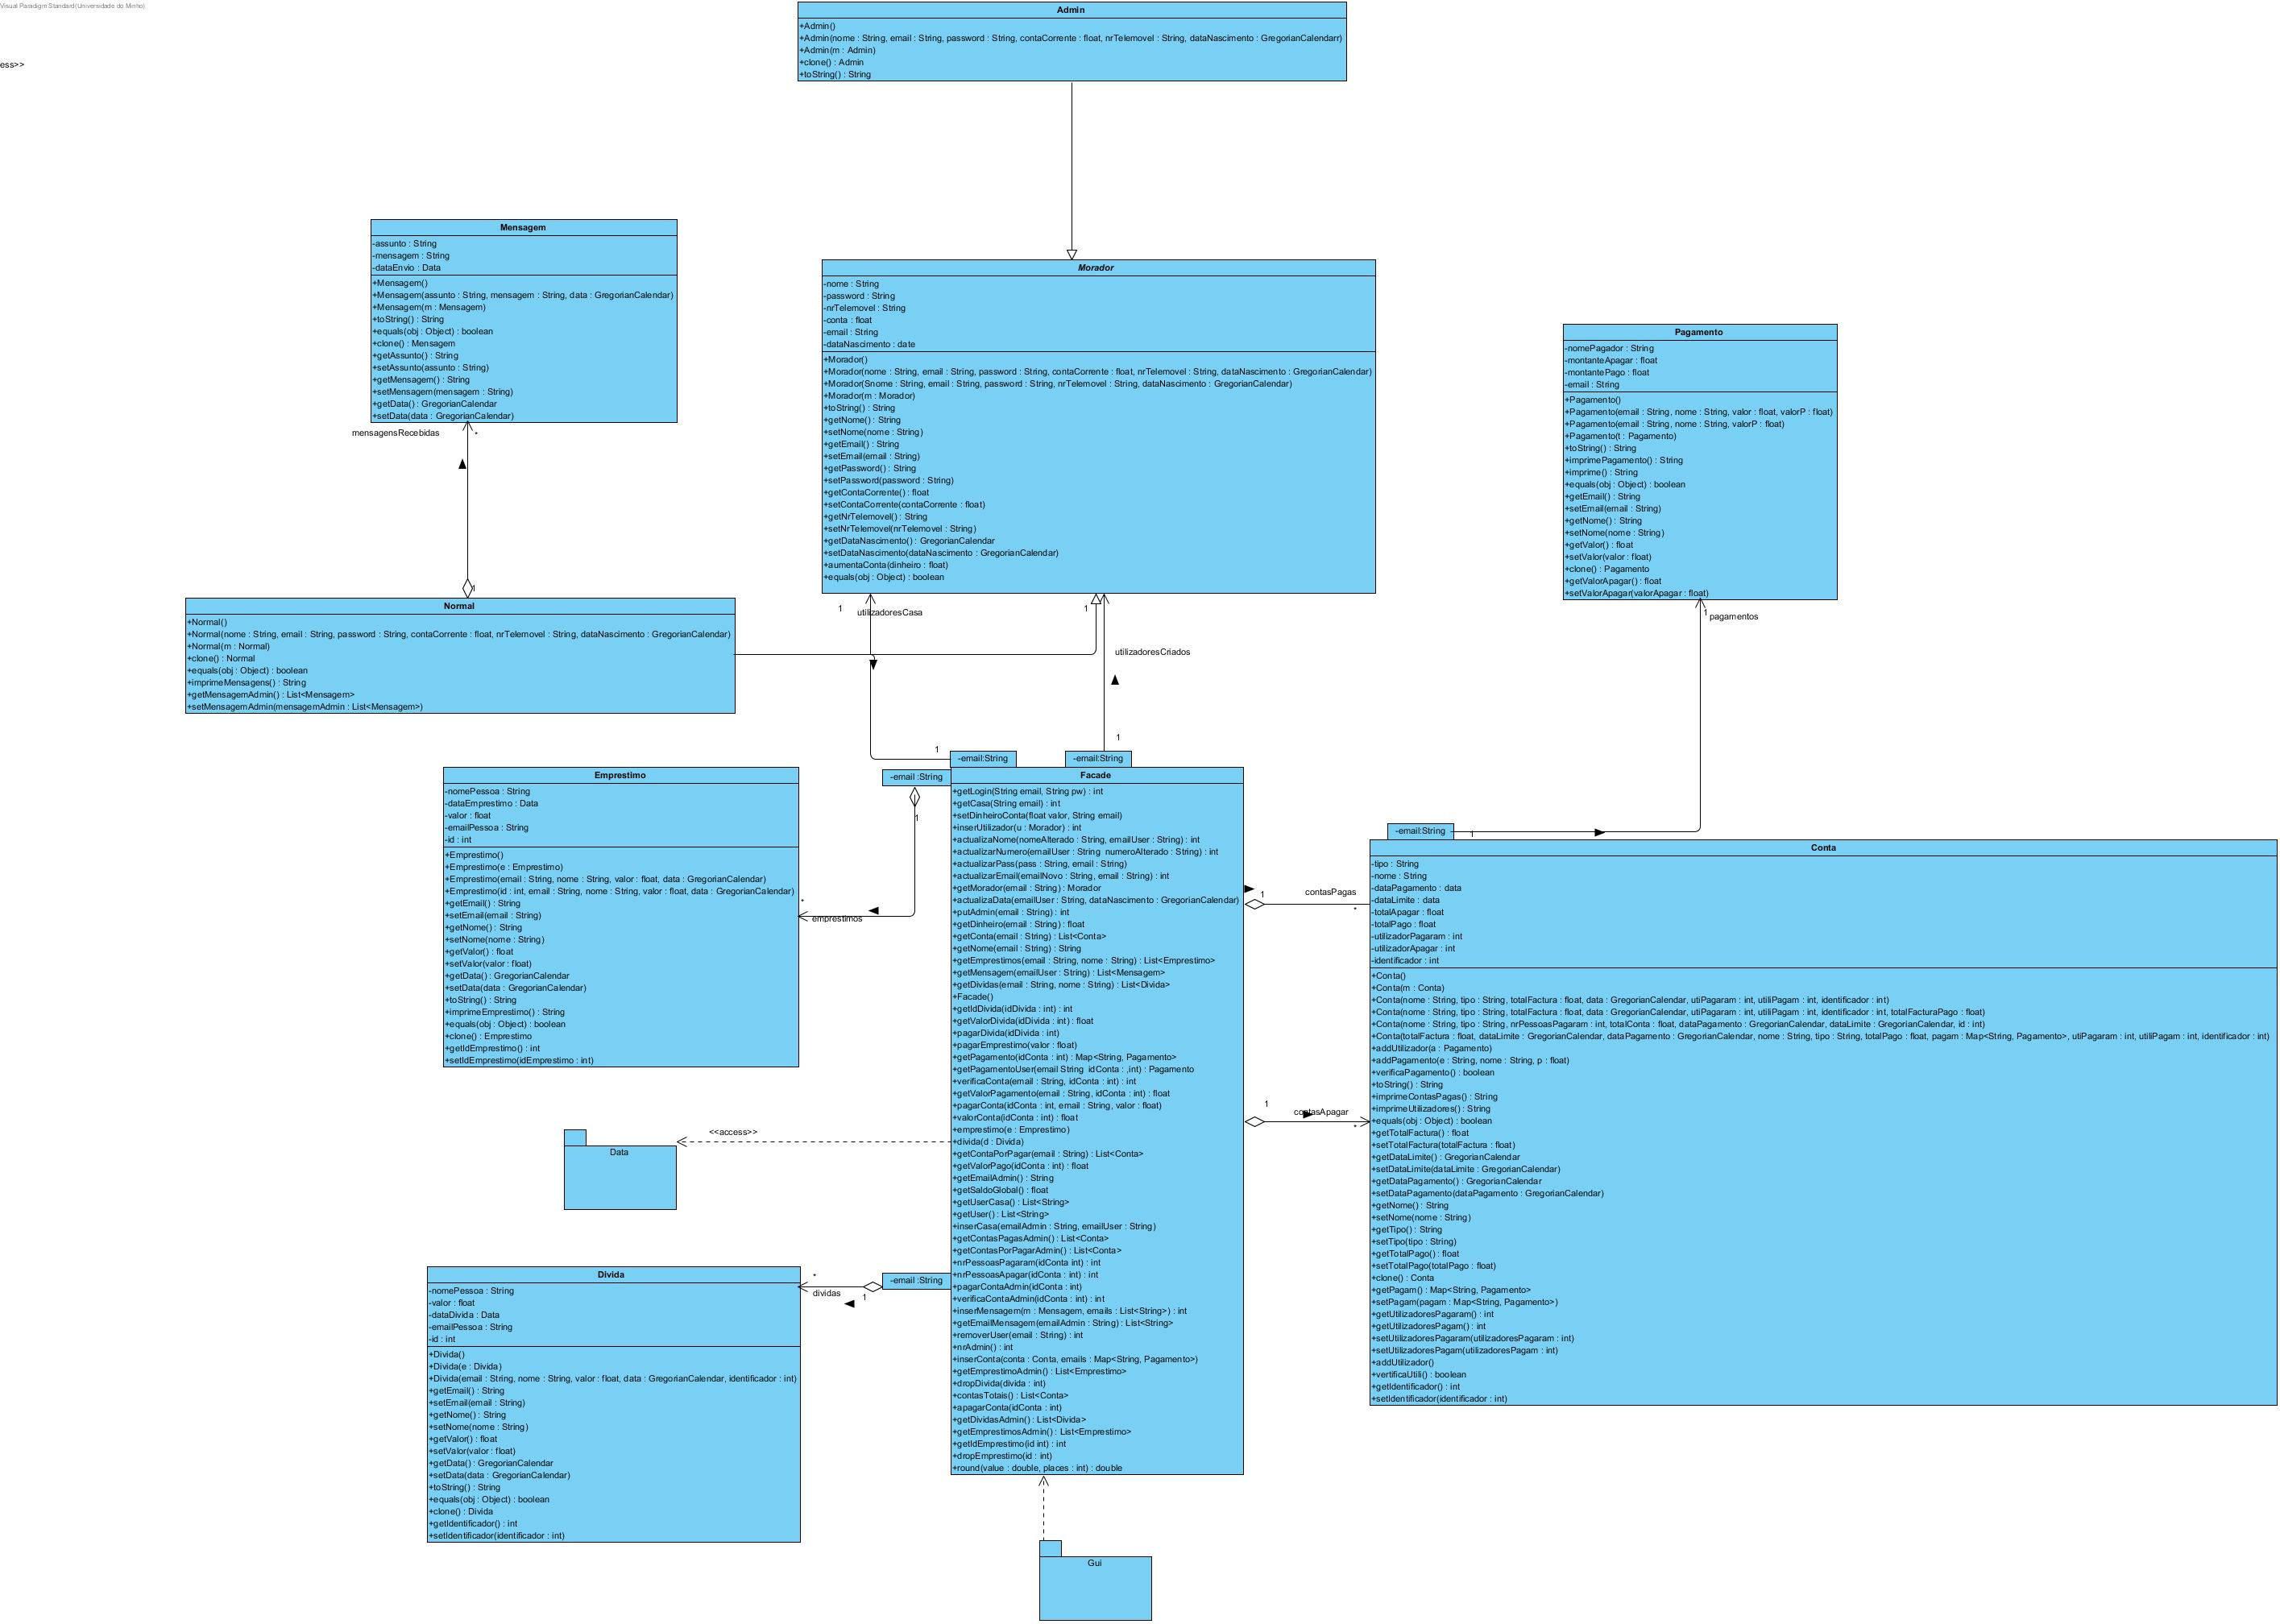
\includegraphics[scale=0.2]{imagens/diagramaClasses/DiagramaClasse}  
	\caption{Diagrama de Classes }  
\end{figure}


\newpage

\section{Modelo de Use Case}
A segunda parte da análise de requisitos corresponde à definição dos use cases, com o objetivo de os aplicar nesta primeira fase deste trabalho prático. Nos use cases, queremos primeiramente, identificar os atores, que serão quem interagirá com o sistema.
Posterior à identificação dos atores, passamos então à identificação dos use cases, isto é, o que se pretende do sistema. No último ponto da visão orientada aos use cases, procedemos à identificação das classes de suporte à realização dos mesmo, que corresponde à especificação da funcionalidade a ser implementada.
Neste sentido, quando definimos um use case, para além de ser uma espécie de documentação, temos de ter em conta que se trata de uma unidade coerente de funcionalidade, um serviço. Define também um comportamento do sistema, sem revelar a estrutura interna, divulgando desta forma, a comunicação entre os atores e o sistema.
O conjunto de todos os use cases acaba por definir pela íntegra, toda a funcionalidade do sistema que decorre na sua essência, do diálogo entre o sistema e os atores, e a responsabilidade de resposta funcional do sistema.


\subsection{Diagrama de Use Case}


\begin{figure}[htb!]
	\centering
	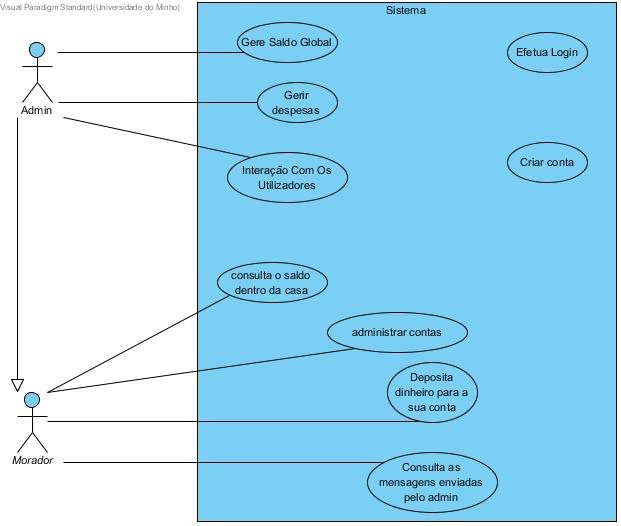
\includegraphics[scale=0.5]{imagens/useCase/UseCase}  
	\caption{Modelo Use Case}  
\end{figure}

\newpage
\subsubsection{Especificação: Gere Saldo Global }

Esta interação pressupõe que o administrador  tenha o login previamente efetuado e desta forma, a visualização do saldo global ao Admin será simples e clara. É então desta forma que o Admin tem acesso ao valor que consta no saldo global, onde esse valor é simplesmente dado a conhecer pelo sistema. O saldo global a que nos referimos é o resultado do somatório de todas as contas correntes de cada morador do apartamento em questão. Este Use Case apenas dá a conhecer ao Admin esse valor.

O use case em formato tabular do Gere saldo Global e o seu respectivo diagrama de sequência é o seguinte:

\begin{figure}[htb!]
	\centering
	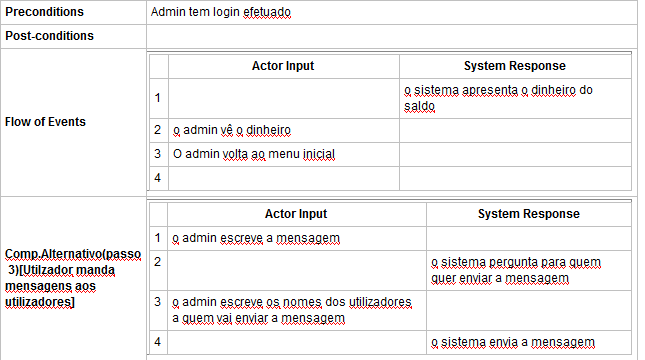
\includegraphics[scale=0.6]{imagens/Especificacoes/geresaldoglobal}  
	\caption{Especificação do Use Case: Gere Saldo Global  }  
\end{figure}

\begin{figure}[htb!]
	\centering
	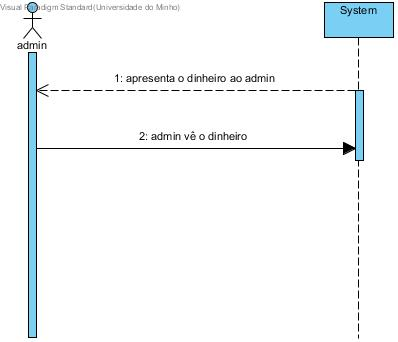
\includegraphics[scale=0.5]{imagens/diagramaSeq/GereSaldoGlobal}  
	\caption{Diagrama de Sequência: Gere Saldo Global}  
\end{figure}


\subsubsection{Especificação: Efetua Login }
Cada morador tem que efetuar Login na aplicação, para tal, é necessário que o indivíduo tenha conta previamente criada. Como em qualquer aplicação, este passo é fundamental e não poderia deixar de o ser no nosso sistema. Para se efetuar o registo do login é solicitado pelo sistema o endereço de email do utilizador em questão para sua validação. Após introduzir o email o sistema requer também o preenchimento da respetiva password. Optamos por colocar um endereço de email ao invés de um username ou um número de telemóvel porque assim poderá existir a possibilidade de futuramente serem enviados para o email dos utilizadores da aplicação, notificações relativas às despesas e ou pagamentos.

\begin{figure}[htb!]
	\centering
	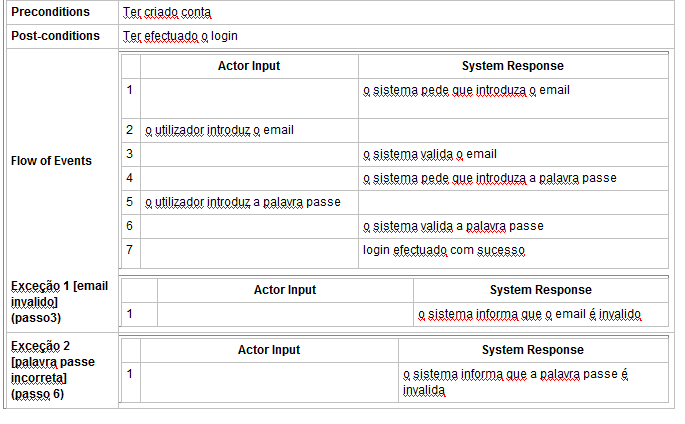
\includegraphics[scale=0.6]{imagens/Especificacoes/efetualogin}  
	\caption{Especificação do Use Case: Efetua Login  }  
\end{figure}


\begin{figure}[htb!]
	\centering
	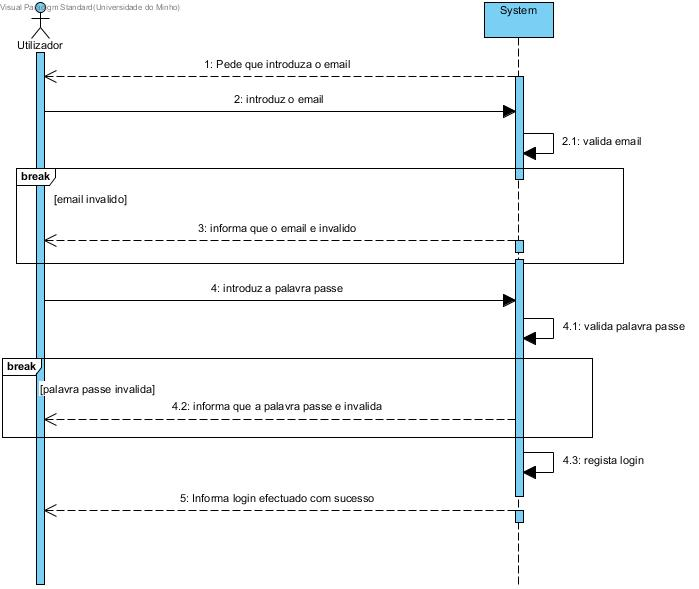
\includegraphics[scale=0.5]{imagens/diagramaSeq/Login}  
	\caption{Diagrama de Sequência: Efetua Login }  
\end{figure}



\newpage

\subsubsection{Especificação: Criar Conta }
Esta interação é uma interação bastante vulgar no sentido em que em praticamente todas as aplicações o ato de “criar conta” é quase obrigatório.  No nosso sistema este passo é fundamental para os utilizadores poderem utilizar a nossa aplicação. Para um utilizador criar conta tem que mencionar determinados dados ao sistema e este tem aceitar estes mesmos dados. Esses dados são simples e optamos por apenas solicitar o nome, data de nascimento, e-mail, número de telemóvel e password.

\begin{figure}[htb!]
	\centering
	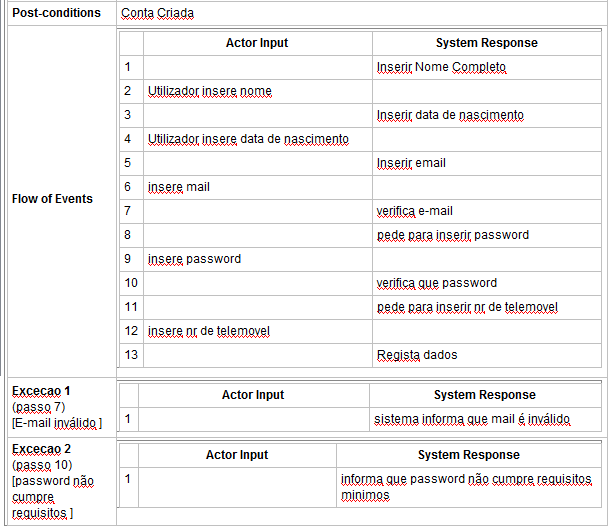
\includegraphics[scale=0.6]{imagens/Especificacoes/criarconta}  
	\caption{Especificação do Use Case: Criar Conta   }  
\end{figure}

\begin{figure}[htb!]
	\centering
	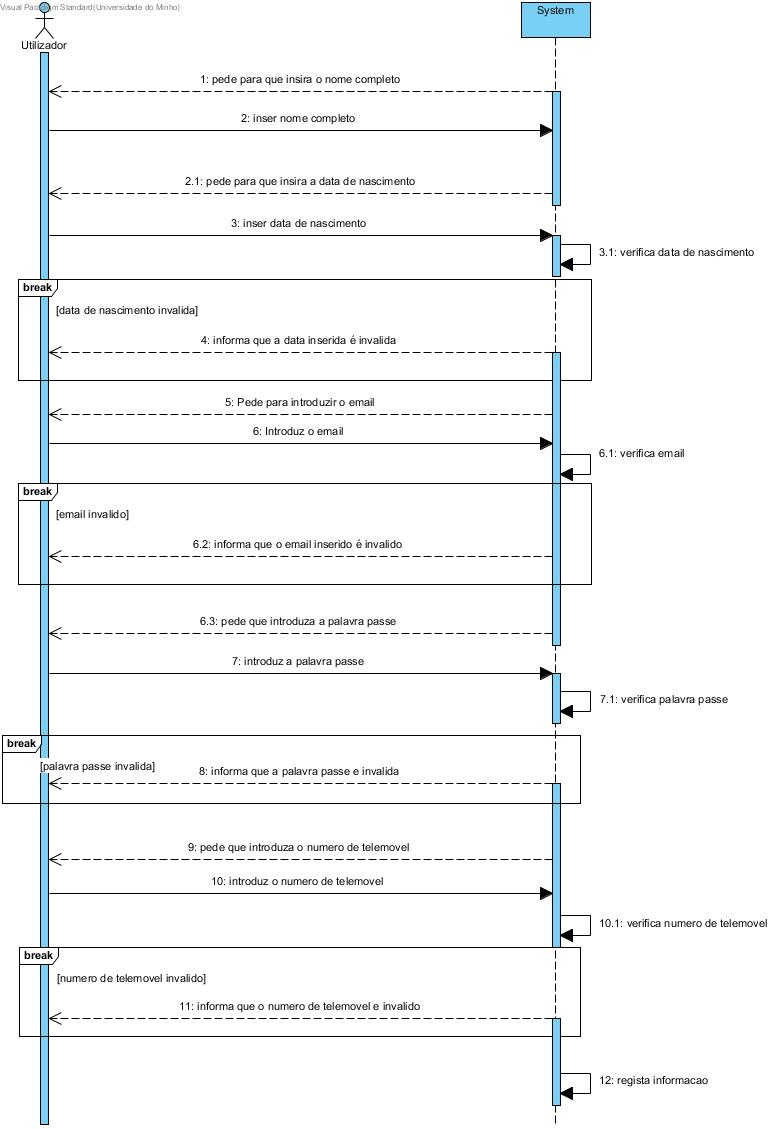
\includegraphics[scale=0.55]{imagens/diagramaSeq/CriarConta}  
	\caption{Diagrama de Sequência: Criar Conta}  
\end{figure}

\newpage \clearpage
\subsubsection{Especificação: Consulta Saldo dentro de casa }
Este use case apenas é útil para a consulta do saldo dentro do apartamento, ou seja, existe a possibilidade de consultar o valor do saldo que consta no apartamento. Cada utilizador que tenta aceder a este saldo, tem que ter o login feito.
\begin{figure}[htb!]
	\centering
	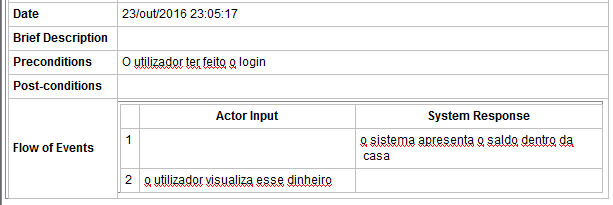
\includegraphics[scale=0.6]{imagens/Especificacoes/consultasaldodentrodecasa}  
	\caption{Especificação do Use Case: Consulta Saldo dentro de Casa   }  
\end{figure}

\begin{figure}[htb!]
	\centering
	\includegraphics[scale=0.5]{imagens/diagramaSeq/ConsultaSaldodeCasa}  
	\caption{Diagrama de Sequência: Consulta saldo de casa  }  
\end{figure}


\subsubsection{Especificação: Deposita Dinheiro para a sua Conta }
Esta especificação foi feita a pensar no depósito da conta corrente de cada morador/utilizador da aplicação, assim como,  a atualização da conta corrente. Basicamente, o sistema solicita que o utilizador adicione determinada quantia na conta corrente e após este procedimento ser efetuado com sucesso a conta corrente surge atualizada. Este processo requer que o utilizador tenha o login efetuado, pois só desta forma é possível aceder a estas especificações.  
\begin{figure}[htb!]
	\centering
	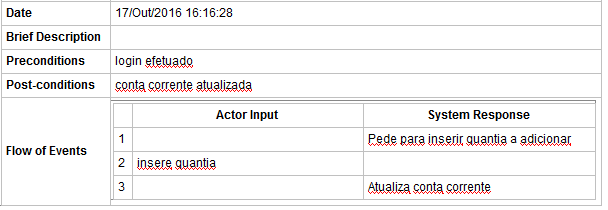
\includegraphics[scale=0.6]{imagens/Especificacoes/depositadinheiro}  
	\caption{Especificação do Use Case: Deposita Dinheiro para a sua conta  }  
\end{figure}

\begin{figure}[htb!]
	\centering
	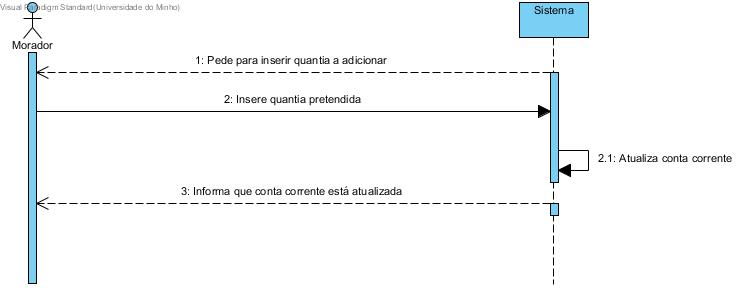
\includegraphics[scale=0.5]{imagens/diagramaSeq/DepositaDinheiroConta}  
	\caption{Diagrama de Sequência: Deposita Dinheiro na Conta}  
\end{figure}


\subsubsection{Especificação: Consulta Mensagens enviadas pelo Administrador }
\begin{figure}[htb!]
	\centering
	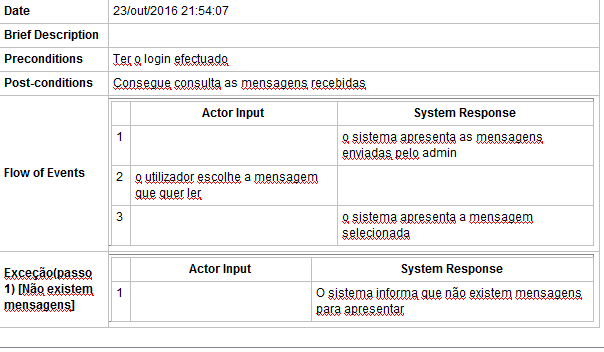
\includegraphics[scale=0.6]{imagens/Especificacoes/consultasmsadmin}  
	\caption{Especificação do Use Case: Consulta Mensagens enviadas pelo Administrador}  
\end{figure}

\begin{figure}[htb!]
	\centering
	\includegraphics[scale=0.5]{imagens/diagramaSeq/ConsultarMensagensdoAdmin}  
	\caption{Diagrama de Sequência: Consulta Mensagens}  
\end{figure}

\newpage

\subsection{Subdiagrama Gerir Despesas}

\begin{figure}[htb!]
	\centering
	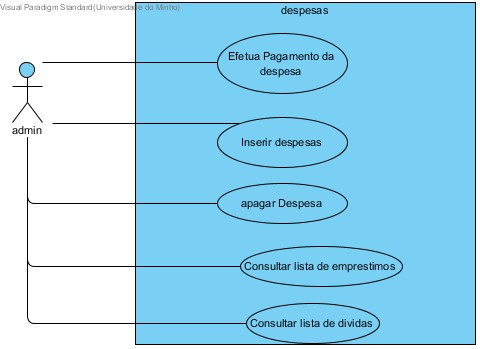
\includegraphics[scale=0.5]{imagens/UseCase/GerirDespesas}  
	\caption{Sub-Diagrama Gerir Despesas }  
\end{figure}

\subsubsection{Especificação: Efetua pagamento da despesa}

De forma a organizar a nossa aplicação apresentamos as despesas que estão por pagar por lista de onde são visualizadas as despesas que estão por pagar e assim fazendo um clique é possível aceder a uma determinada fatura seleccionada pelo utilizador.  A despesa em falta é automaticamente descontada ao saldo global do apartamento em causa. Deste modo, sabemos sempre se existem faturas por pagar e o saldo é atualizado no imediato. Claro está , que é necessário que o valor do saldo seja sempre igual ou superior aos valores indicados nas faturas.


\begin{figure}[htb!]
	\centering
	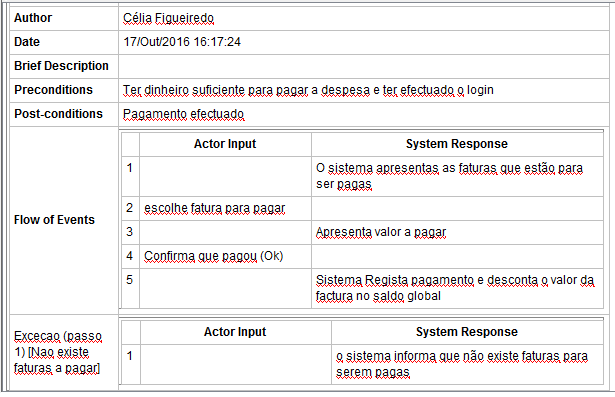
\includegraphics[scale=0.6]{imagens/Especificacoes/efetuapagdespesa}  
	\caption{Especificação do Use Case:Efetua Pagamento da despesa  }  
\end{figure}

\begin{figure}[htb!]
	\centering
	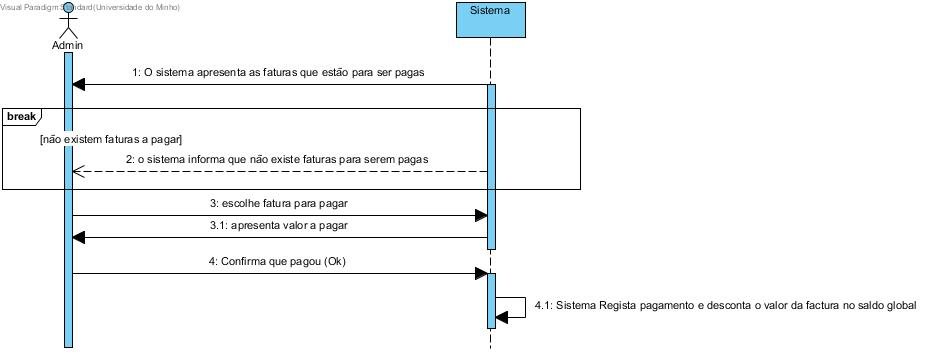
\includegraphics[scale=0.5]{imagens/diagramaSeq/EfetuaPagamentoDespesa}  
	\caption{Diagrama de Sequência: Administrador efetua pagamento da despesa }  
\end{figure}


\begin{figure}[htb!]
	\centering
	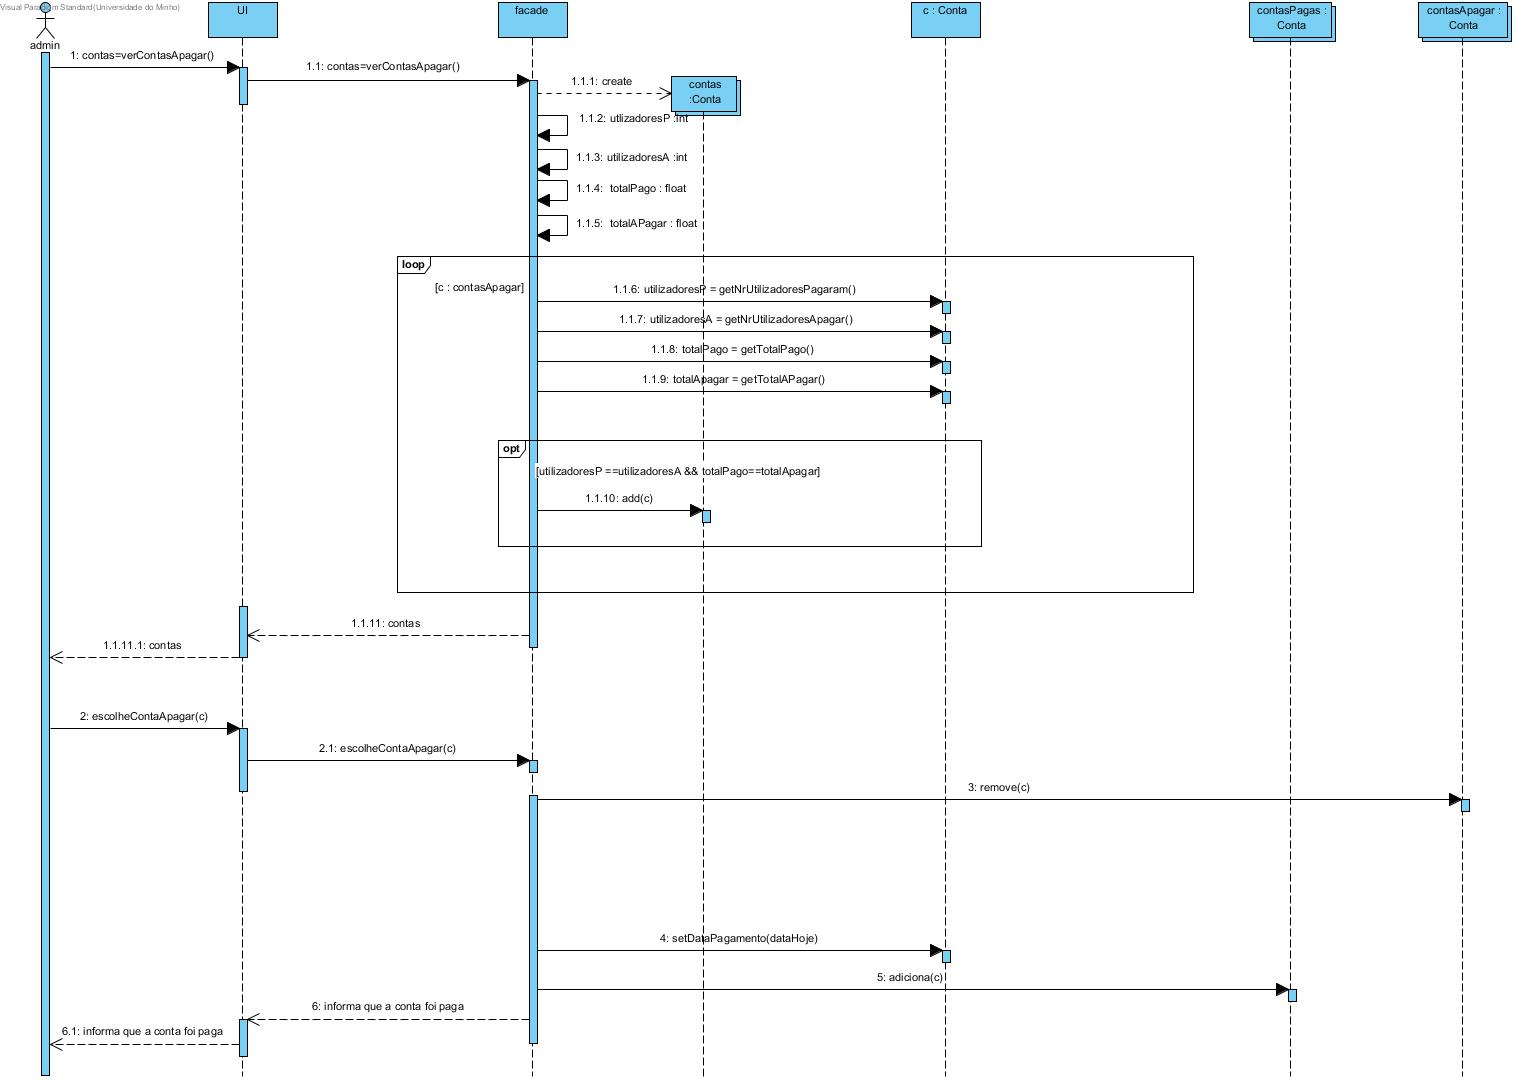
\includegraphics[scale=0.345]{imagens/diagramaIt/AdminPagaFactura}  
	\caption{Diagrama de Iteração: Administrador efetua pagamento }  
\end{figure}


\newpage
\subsubsection{Especificação: Inserir Despesa}

Cabe ao administrador fazer as inserções das despesas no sistema. Para que cada inserção seja feita com sucesso têm que ser bem introduzidas e aceites pelo sistema, colocando a data, o nome e os valores de cada fatura válidos.
É também tarefa do administrador decidir que percentagem cada morador registado tem que pagar de cada fatura/despesa.

\begin{figure}[htb!]
	\centering
	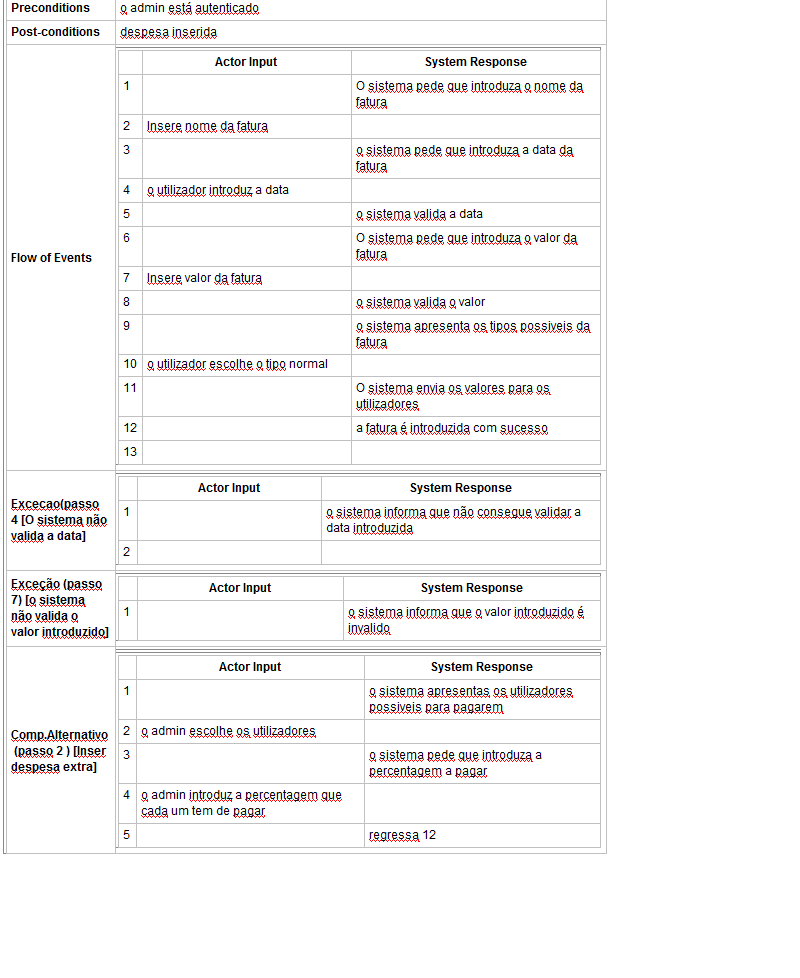
\includegraphics[scale=0.8]{imagens/Especificacoes/inserirdespesas}  
	\caption{Especificação do Use Case: Inserir Despesas}  
\end{figure}


\begin{figure}[htb!]
	\centering
	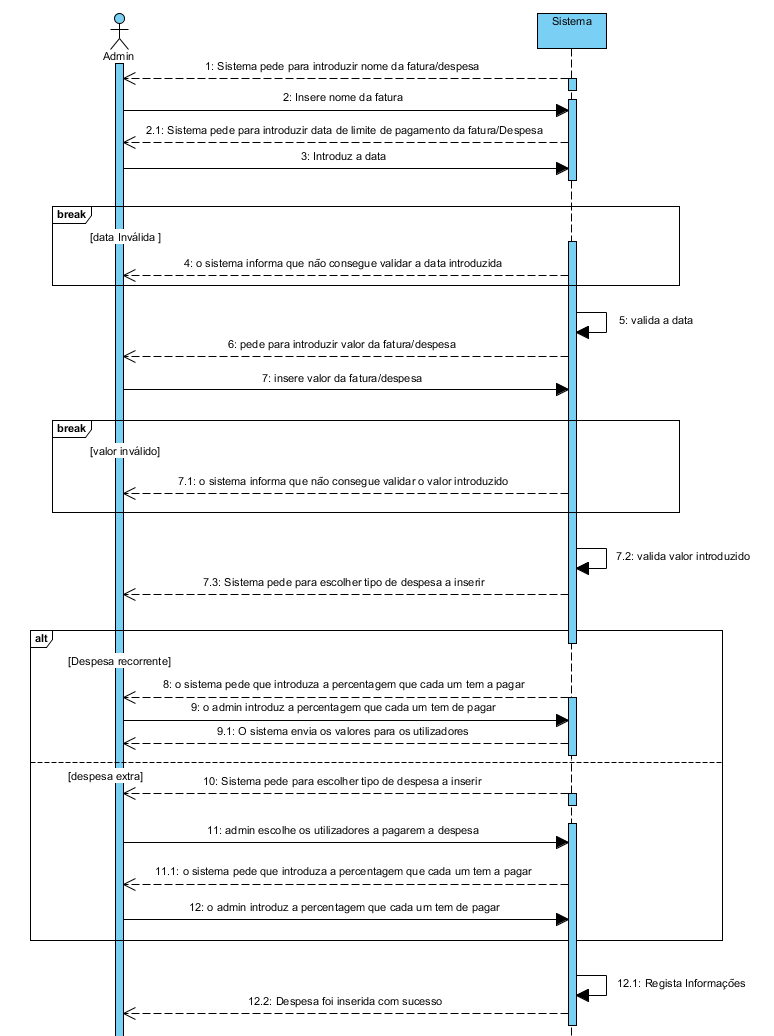
\includegraphics[scale=0.5]{imagens/DiagramaSeq/InserirDespesa}  
	\caption{Diagrama de Sequência: Inserir Despesa}  
\end{figure}

\newpage \clearpage

\subsubsection{Especificação: Apagar Despesa}

O administrador tanto insere as despesas no sistema como as elimina. Temos apenas que ter em consideração que é condição necessária que o admin tenha o login efetuado e a partir daqui o sistema apresenta a listas das despesas por pagar o administrador apenas selecciona aquela que efetivamente pretende que seja eliminada.

\begin{figure}[htb!]
	\centering
	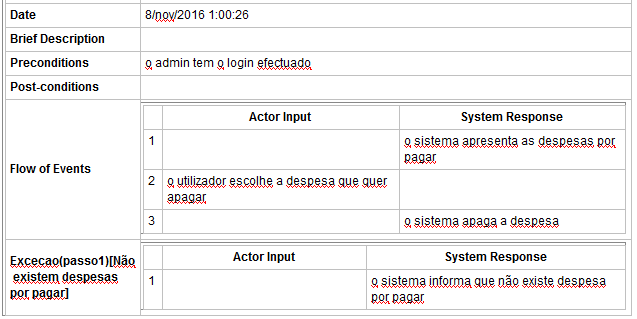
\includegraphics[scale=0.6]{imagens/Especificacoes/apagardespesa}  
	\caption{Especificação do Use Case: Apagar Despesa}  
\end{figure}

\begin{figure}[htb!]
	\centering
	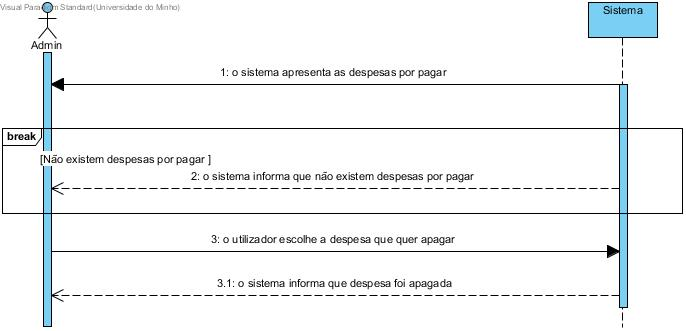
\includegraphics[scale=0.5]{imagens/diagramaSeq/ApagarDespesa}  
	\caption{Diagrama de Sequência: Apagar Despesa}  
\end{figure}

\newpage
\subsection{Subdiagrama Administrar Contas}
\begin{figure}[htb!]
	\centering
	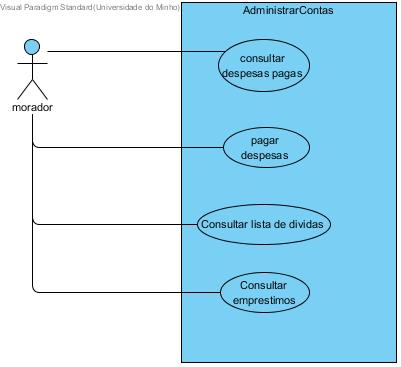
\includegraphics[scale=0.6]{imagens/UseCase/despesasMorador}  
	\caption{Subdiagrama: Administrar Contas }  
\end{figure}



\subsubsection{Especificação: Consultar despesas pagas }
Esta é uma consulta feita pelo administrador. Fica possível a consulta de cada uma das despesas que já foram pagas. Esta interação apenas serve para consultar informação. O sistema apresenta todos os detalhes da fatura previamente seleccionada pelo admin. 
Como o próprio nome do subdiagrama indica, trata-se de administrar contas. 

\begin{figure}[htb!]
	\centering
	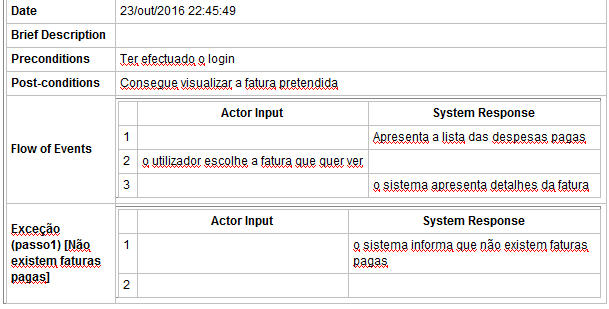
\includegraphics[scale=0.6]{imagens/Especificacoes/consultardespesaspagas}  
	\caption{Especificação do Use Case: Consultar Despesas Pagas}  
\end{figure}

\begin{figure}[htb!]
	\centering
	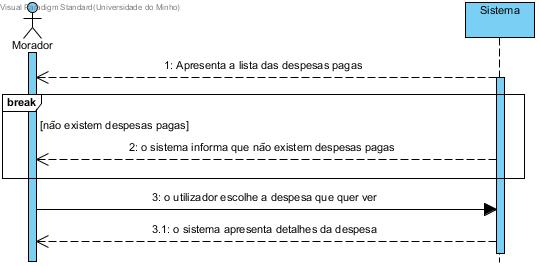
\includegraphics[scale=0.6]{imagens/DiagramaSeq/ConsultarDespesasPagas}  
	\caption{Diagrama de Sequência: Consultar Despesas pagas }  
\end{figure}


\newpage
\subsubsection{Especificação: Pagar Despesas }
É nesta especificação que está descrito como é que todos os pagamentos da nossa aplicação são efetivamente pagos.
Cada utilizador, previamente registado e com login feito selecciona a conta que pretende pagar e procede ao pagamento em questão. O sistema após validar este pagamento atualiza a informação e coloca-a visível. 

\begin{figure}[htb!]
	\centering
	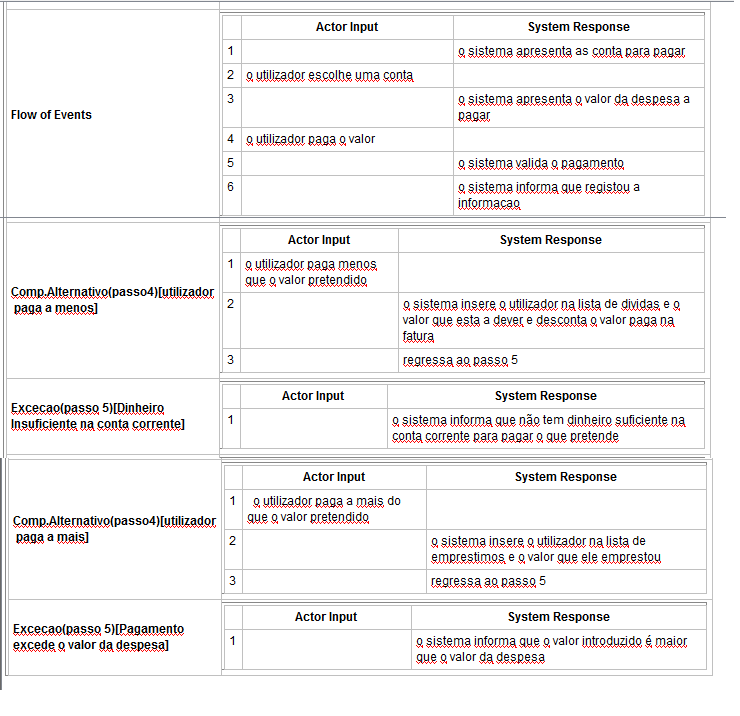
\includegraphics[scale=0.6]{imagens/Especificacoes/pagardespesas}  
	\caption{Especificação do Use Case: Pagar Despesas}  
\end{figure}


\begin{figure}[htb!]
	\centering
	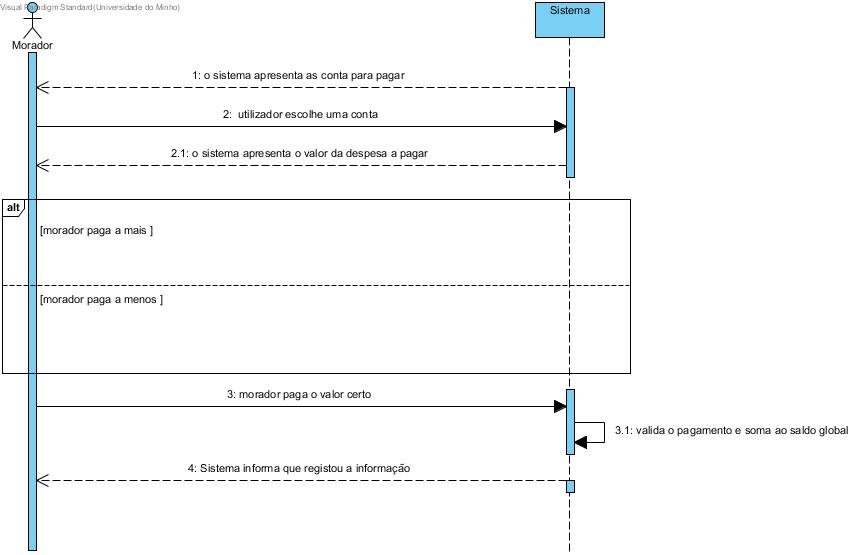
\includegraphics[scale=0.5]{imagens/DiagramaSeq/PagarDespesa}  
	\caption{Diagrama de Sequência: Utilizador paga despesa}  
\end{figure}


\begin{figure}[htb!]
	\centering
	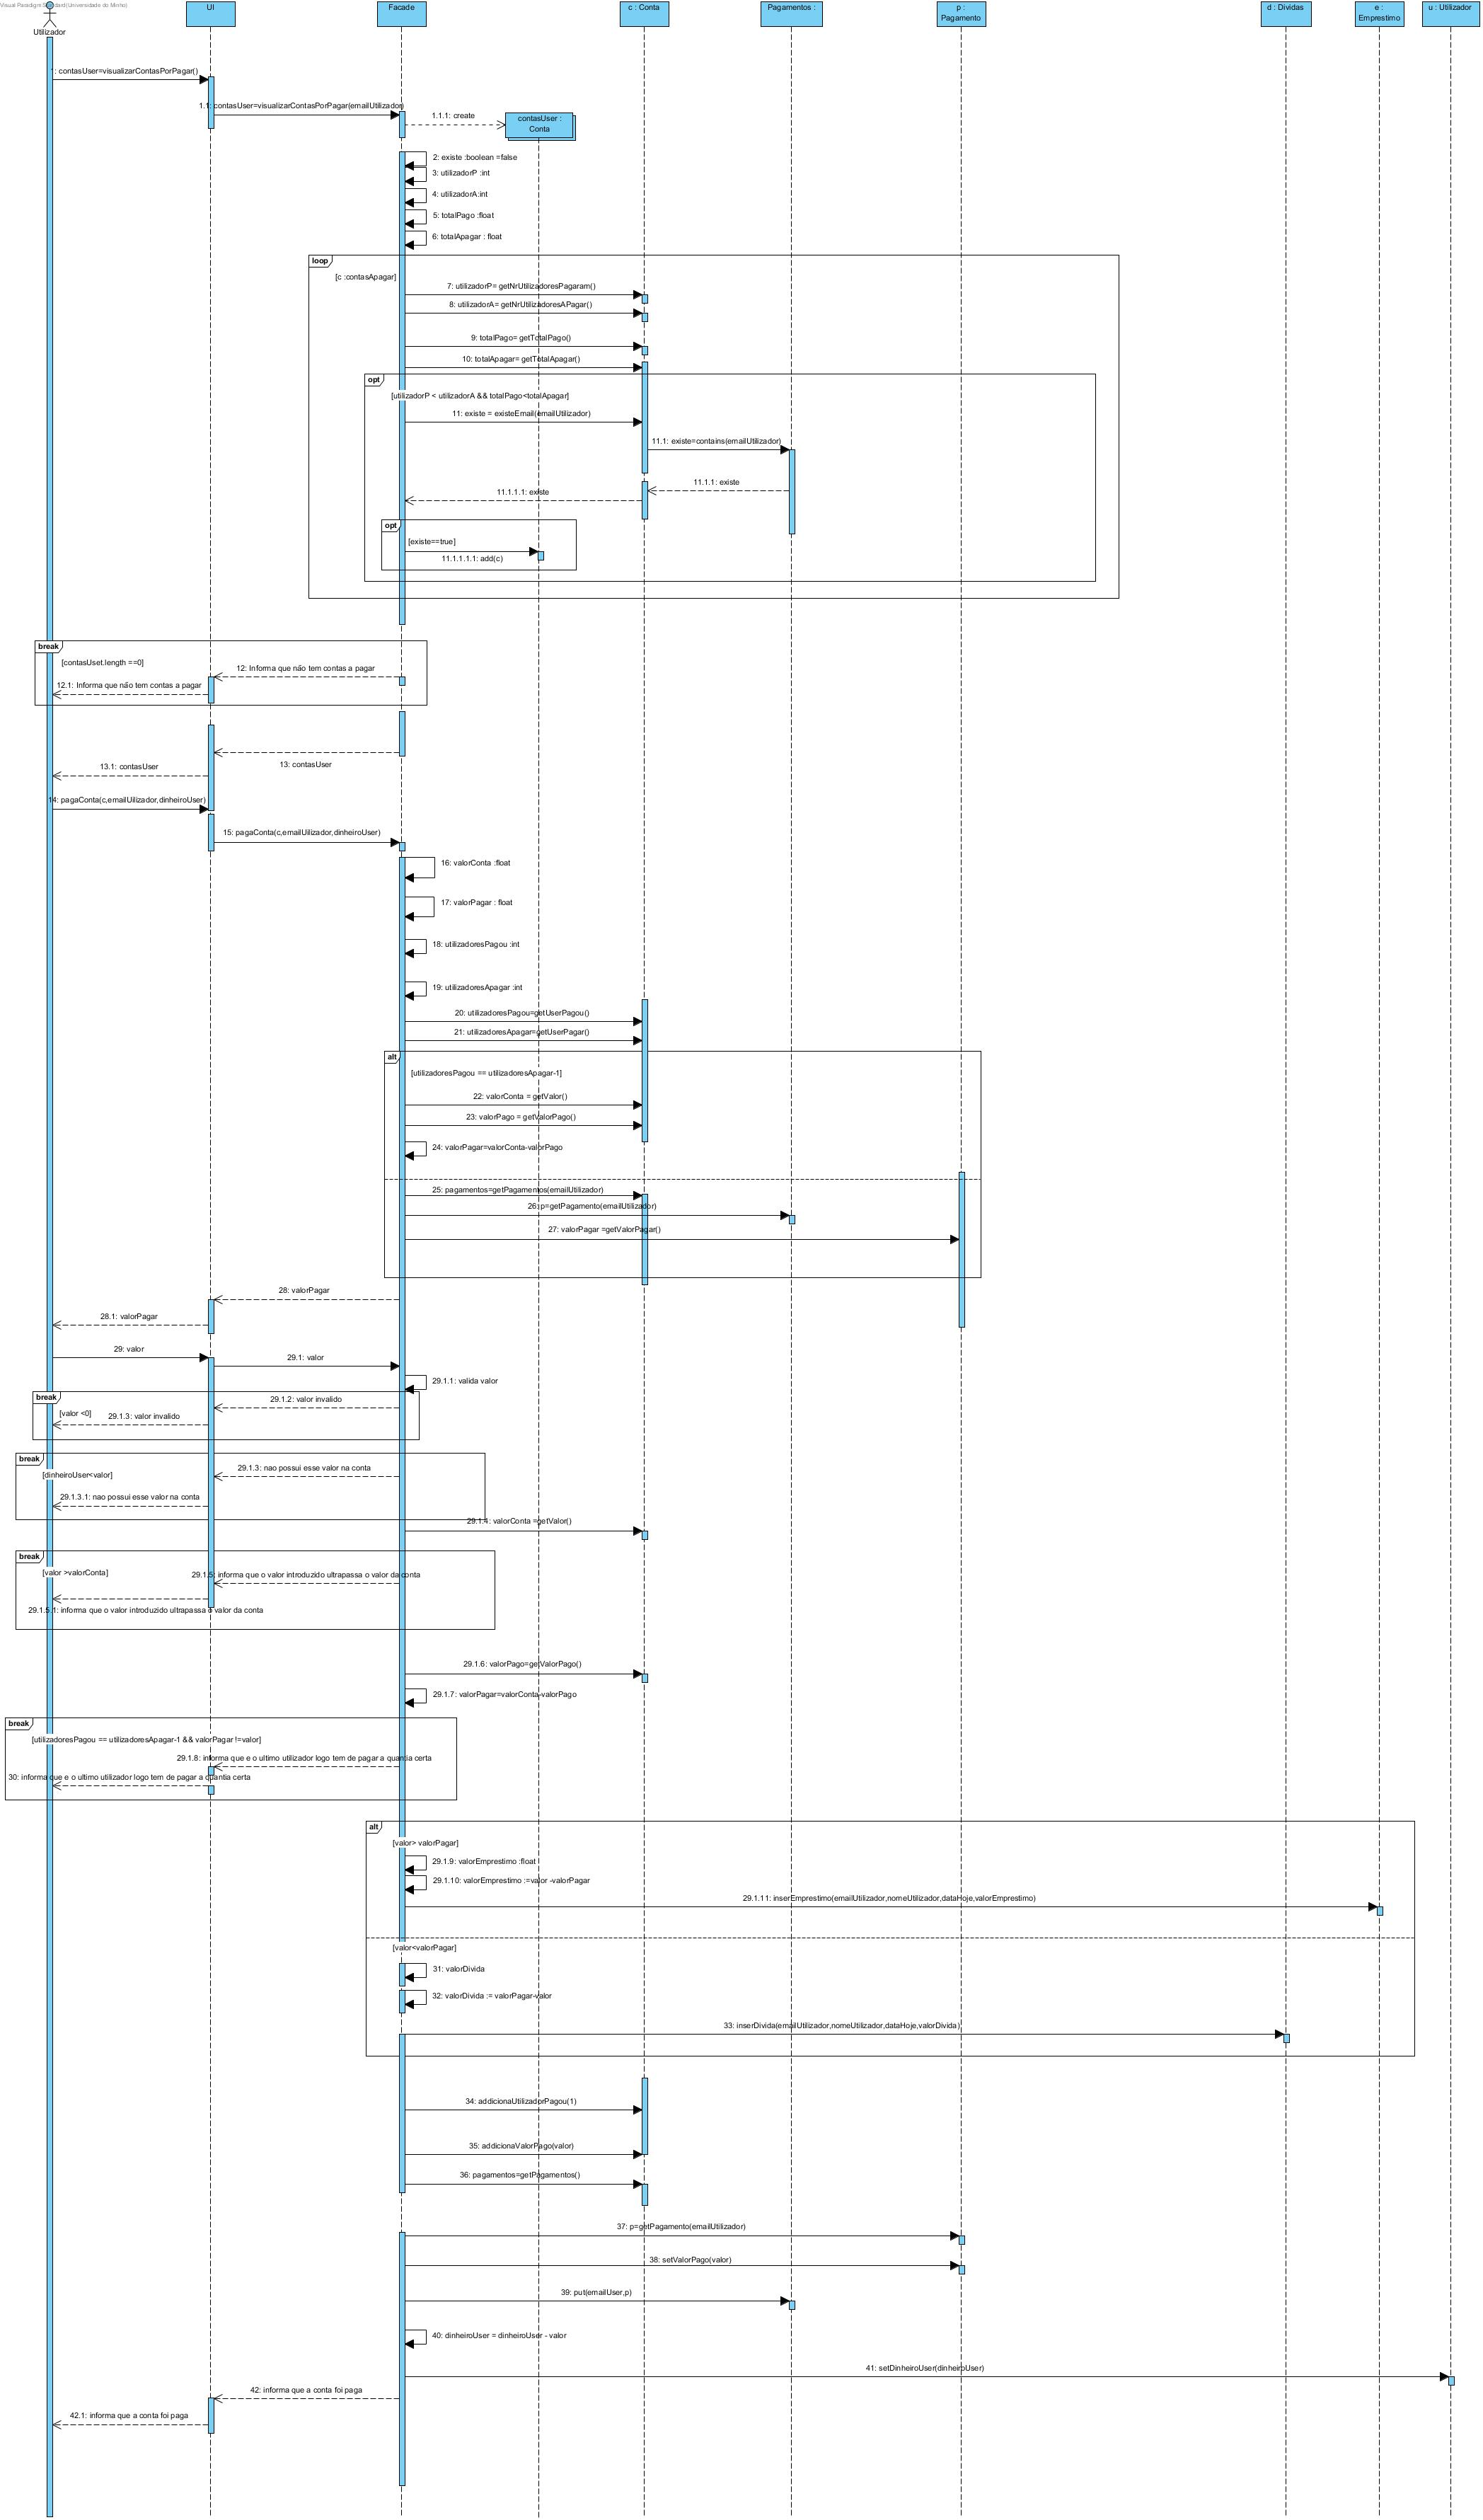
\includegraphics[scale=0.18]{imagens/DiagramaIt/UtilizadorPagaFactura}  
	\caption{Diagrama de Iteração: Utilizador Paga Despesas}  
\end{figure}

\newpage \clearpage

\subsubsection{Especificação: Consultar Empréstimos }

Nesta especificação o utilizador tem a vantagem de aceder à lista de empréstimos, ou seja, consegue através da aplicação visualizar os valores que emprestou a outros moradores do apartamento, previamente registados na aplicação. 

\begin{figure}[htb!]
	\centering
	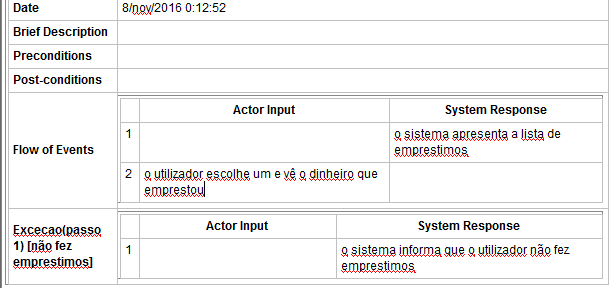
\includegraphics[scale=0.7]{imagens/Especificacoes/consultaremprestimos}  
	\caption{Especificação do Use Case: Consultar Empréstimos}  
\end{figure}

\begin{figure}[htb!]
	\centering
	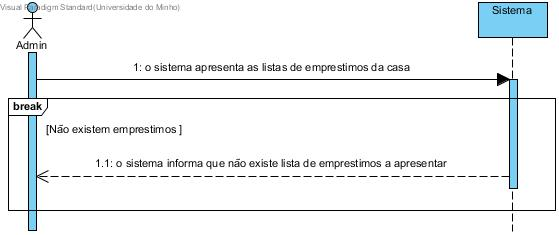
\includegraphics[scale=0.5]{imagens/diagramaSeq/ConsultarListaEmprestimos}  
	\caption{Diagrama de Sequência: Consulta lista de empréstimos}  
\end{figure}

\newpage
\subsubsection{Especificação: Consultar Lista de Dívidas }
Paralelamente ao que foi referido na especificação do use case de “consultar lista de emprestimos”, nesta secção é possível ter acesso à lista de dívidas. Por dívidas entende-se dinheiro que o morador deve à casa, neste caso a alguém que colocou o dinheiro por ele. 
A consulta de dívidas permite que cada utilizador tenha acesso à lista de dívidas e valores por pagar, desta forma tem sempre as contas com os valores exatos em dívida sem ter que fazer cálculos e arredondamentos.

\begin{figure}[htb!]
	\centering
	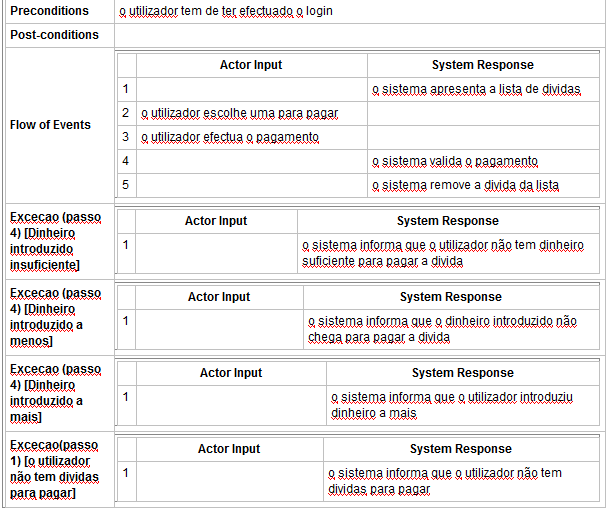
\includegraphics[scale=0.7]{imagens/Especificacoes/consultarlistadedividas}  
	\caption{Especificação do Use Case: Consultar lista de dividas}  
\end{figure}


\begin{figure}[htb!]
	\centering
	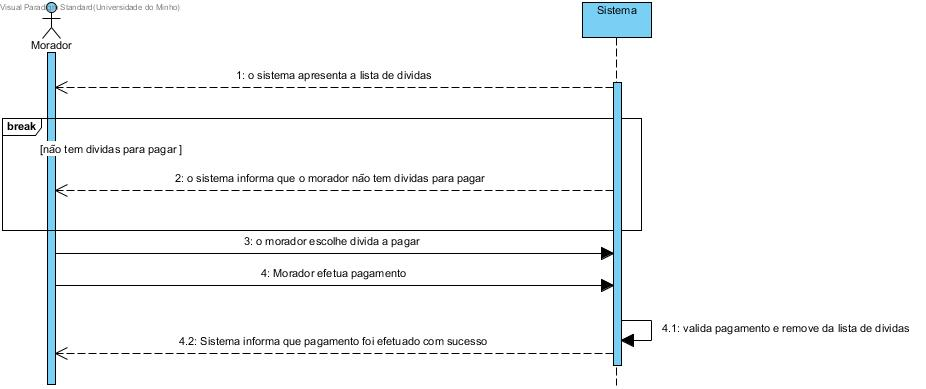
\includegraphics[scale=0.6]{imagens/diagramaSeq/ConsultaListaDividas}  
	\caption{Diagrama de Sequência: Consulta lista de dividas}  
\end{figure}


\newpage

\subsection{Subdiagrama Interação com os Utilizadores}
A interação com os utilizadores da aplicação torna a experiência mais interessante e motivadora. 
\begin{figure}[htb!]
	\centering
	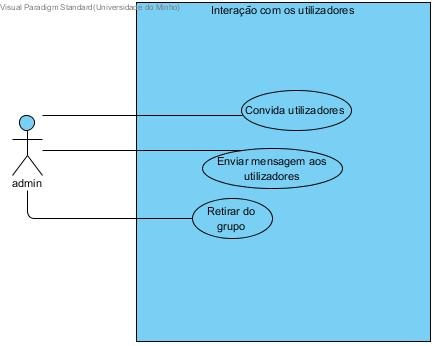
\includegraphics[scale=0.6]{imagens/UseCase/InteracaoComOsUtilizadores}  
	\caption{Subdiagrama: Interação com os utilizadores }  
\end{figure}

\subsubsection{Especificação: Convida Utilizadores }
É através do email que um utilizador previamente registado convida outros a pertencerem ao “grupo” e a começarem a participar nas despesas do apartamento. O novo membro é notificado e de imediato pode proceder ao seu registo e efetuar login. 

\begin{figure}[htb!]
	\centering
	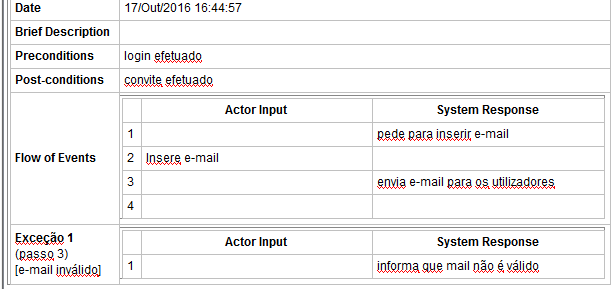
\includegraphics[scale=0.7]{imagens/Especificacoes/convidautilizadores}  
	\caption{Especificação do Use Case: Convida Utilizadores}  
\end{figure}

\begin{figure}[htb!]
	\centering
	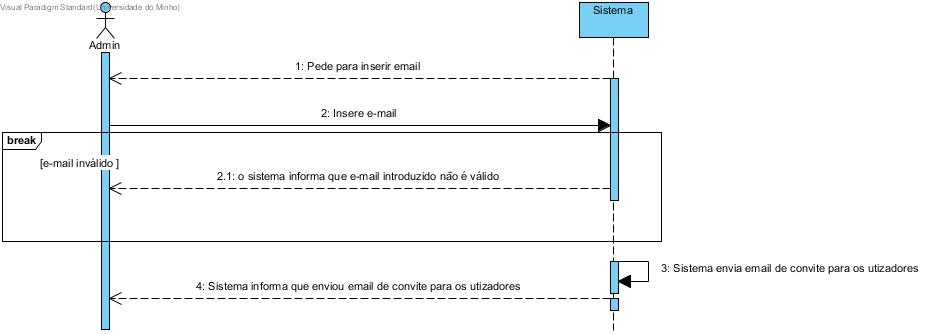
\includegraphics[scale=0.5]{imagens/diagramaSeq/ConvidaUtilizadores}  
	\caption{Diagrama de Sequência: Convida Utilizadores }  
\end{figure}

\begin{figure}[htb!]
	\centering
	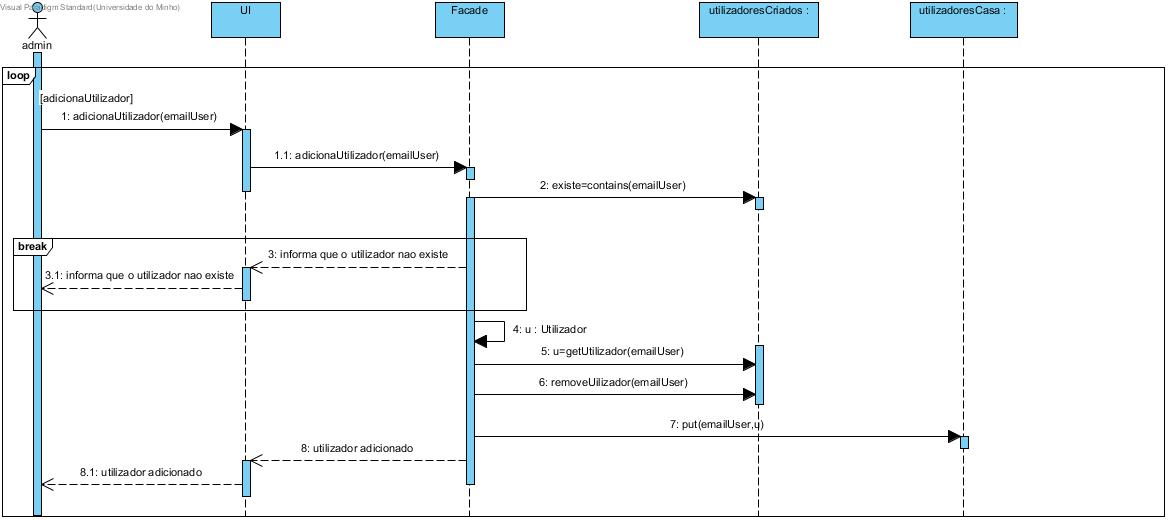
\includegraphics[scale=0.46]{imagens/diagramaIt/AdicionarUtilizadorGrupo}  
	\caption{Diagrama de Iteração: Convida Utilizadores }  
\end{figure}



\newpage \clearpage

\subsubsection{Especificação: Envia Mensagens aos Utilizadores }
O administrador da aplicação tem acesso à lista de utilizadores que estão aptos a receber mensagens. O mesmo escolhe a quem pretende enviar uma mensagem e envia. O sistema apenas confirma o envio. Este processo pode ser enviado aos utilizadores que o administrador quiser.

\begin{figure}[htb!]
	\centering
	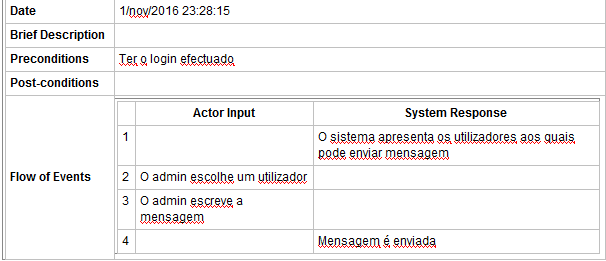
\includegraphics[scale=0.7]{imagens/Especificacoes/enviasmsutilizadores}  
	\caption{Especificação do Use Case: Envia Mensagens aos Utilizadores}  
\end{figure}



\subsubsection{Especificação: Retirar do grupo }
O administrador consegue remover da aplicação os membros que de uma forma ou de   outra já não pertencem ao grupo.  O sistema apresenta a lista dos moradores registados e apenas é seleccionado o membro a excluir. 

\begin{figure}[htb!]
	\centering
	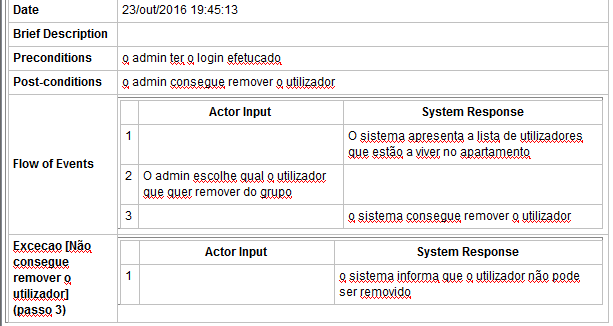
\includegraphics[scale=0.7]{imagens/Especificacoes/retirardogrupo}  
	\caption{Especificação do Use Case: Retirar do grupo}  
\end{figure}

\begin{figure}[htb!]
	\centering
	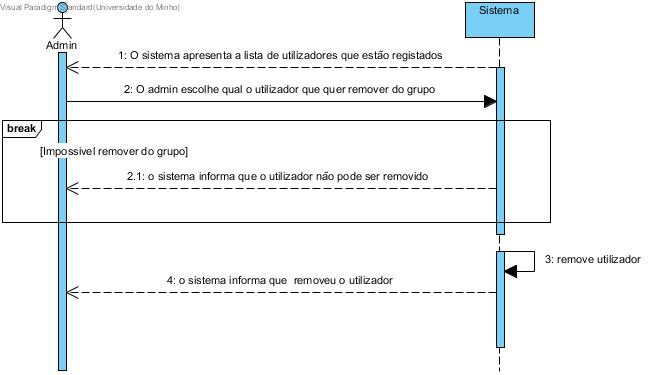
\includegraphics[scale=0.5]{imagens/DiagramaSeq/RetirarDoGrupo}  
	\caption{Diagrama de Sequência: Administrador Remove do Grupo}  
\end{figure}

\begin{figure}[htb!]
	\centering
	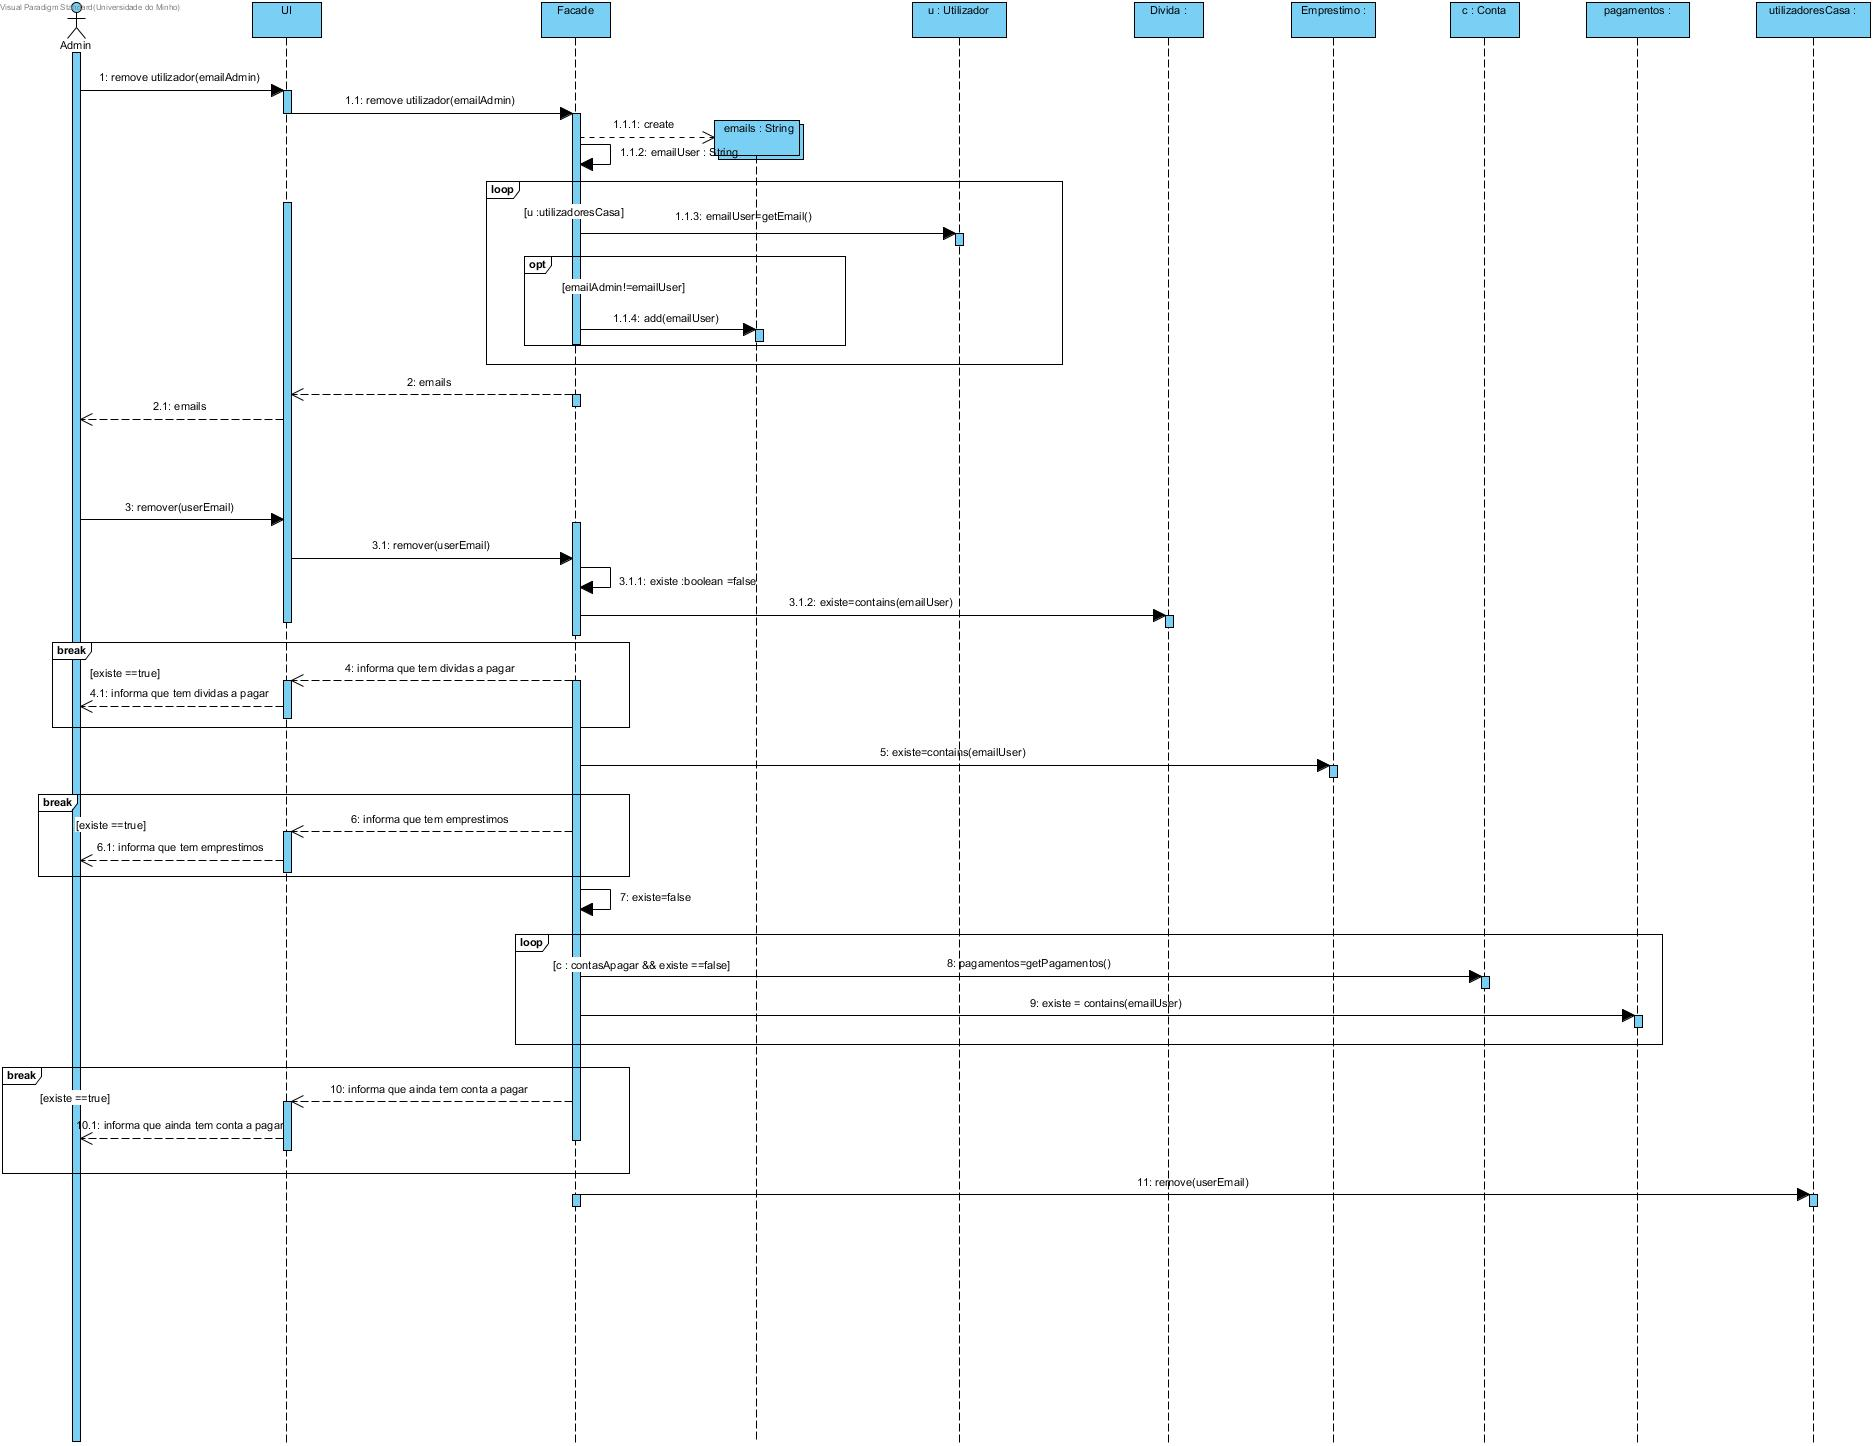
\includegraphics[scale=0.27]{imagens/DiagramaIt/AdminRemoveDoGrupo}  
	\caption{Diagrama de Iteração: Administrador Remove do Grupo}  
\end{figure}


\chapter{Implementação e Instalação do Sistema}

\section{Diagrama de Instalação}

Os dois grandes subsistemas da aplicação desenvolvida são o computador do utilizador e o servidor de base de dados. A comunicação é estabelecida por TCP/IP. O programa é uma aplicação Java, e para a apresentação gráfica ao utilizador, é usado JavaSwing. Para ser possível a comunicação entre a aplicação em Java e a base de dados MySQL, recorre-se à interface JDBC \footnote{Java Database Connectivity} . 

\begin{figure}[htb!]
	\centering
	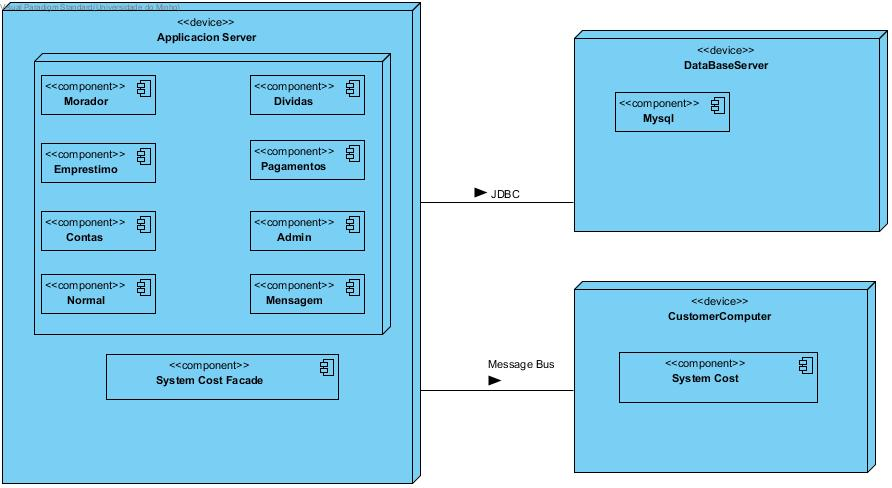
\includegraphics[scale=0.4]{imagens/DiagramInstalacao/DeploymentDiagram}  
	\caption{Diagrama de Instalação ou Deployment Diagram}  
\end{figure}

\newpage

Os três principais pacotes definidos são \textit{Presentation}, que trata da apresentação gráfica, em \textit{Java Swing}; \textit{Business}, que contém toda a lógica de negócio; e \textit{Data}, responsável pela ligação à base de dados. A camada de apresentação comunica com a camada de lógica de negócio a partir da classe
SGD (Sistema de Gestão de Despesas), que desempenha a função de facade.
Não existe qualquer tipo de comunicação feita diretamente entre a camada de
apresentação e a camada de dados. A comunicação entre o package \textit{Business}
e a persistência de Dados é feita recorrendo às várias classes \textit{DAO} implementadas no \textit{Package Data}, que comunicam com a base de dados \textit{MySQL}.

\begin{figure}[htb!]
	\centering
	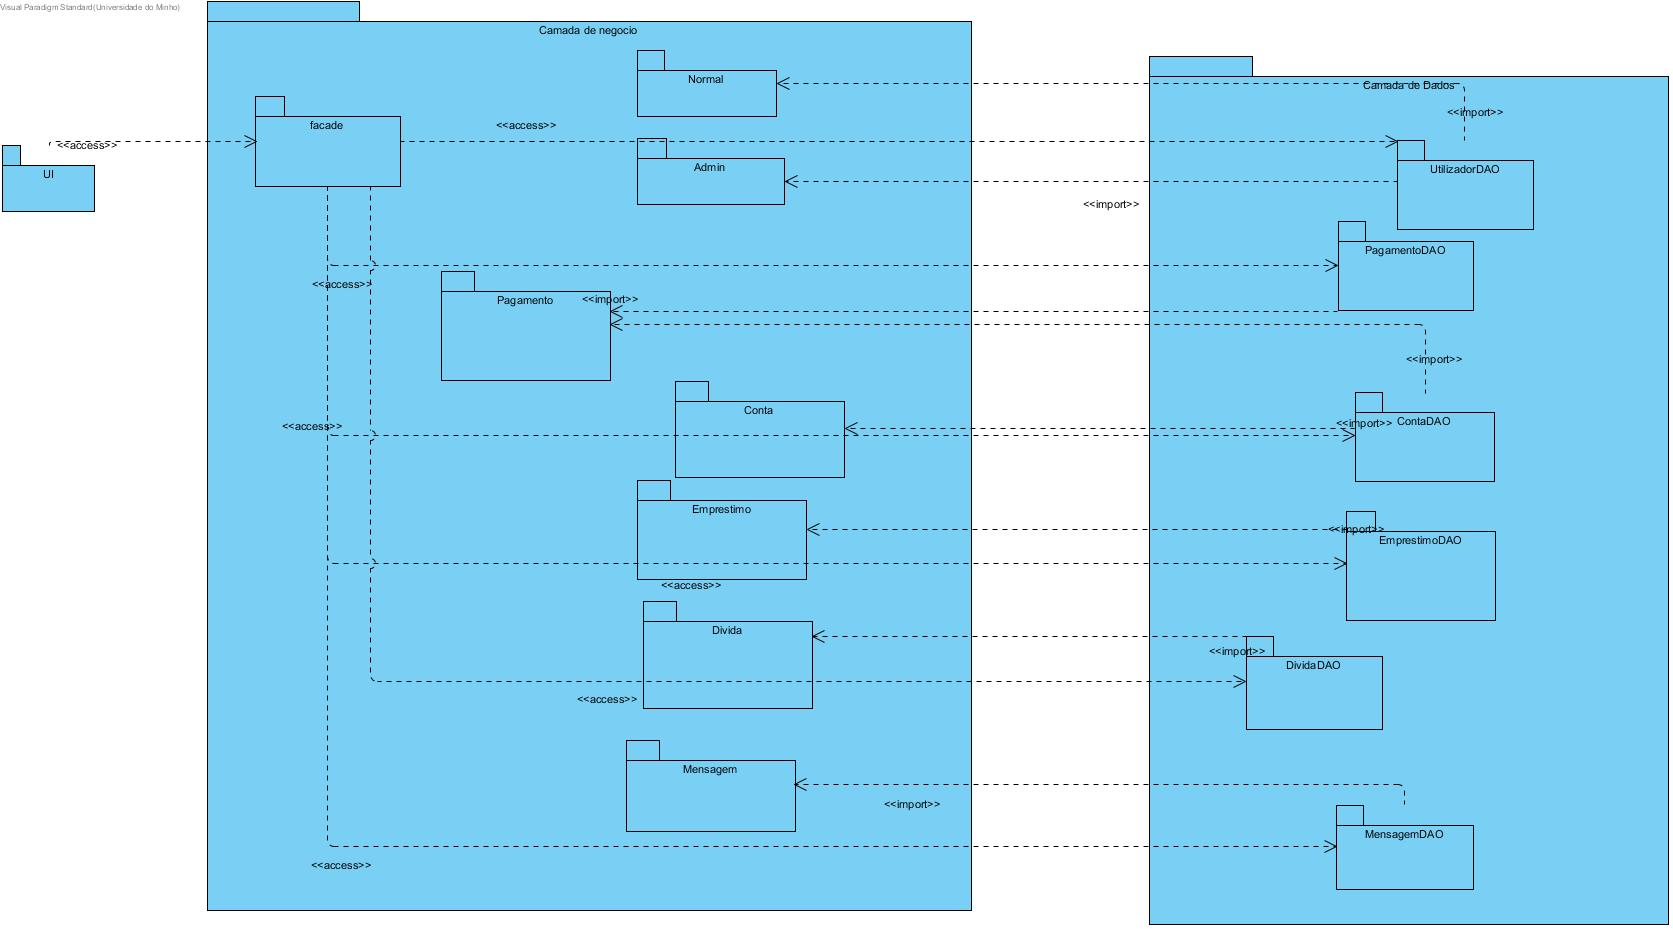
\includegraphics[scale=0.35]{imagens/DiagramInstalacao/PackageDiagram}  
	\caption{Diagrama de Pacotes}  
\end{figure}

\newpage

\chapter{Interface do Sistema Gestão de Despesas - SGD}
\section{Máquinas de Estado}
\subsection{Efetuar Login}

\begin{figure}[htb!]
	\centering
	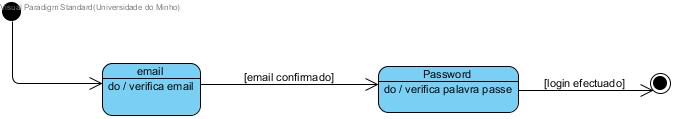
\includegraphics[scale=0.7]{imagens/maqEstados/Login}  
	\caption{Máquina de Estados: Efetuar Login}  
\end{figure}


\subsection{Criar Conta}
\begin{figure}[htb!]
	\centering
	\includegraphics[scale=0.55]{imagens/maqEstados/"Criar Conta"}  
	\caption{Máquina de Estados: Criar Conta}  
\end{figure}

\subsection{Convidar Utilizadores}
\begin{figure}[htb!]
	\centering
	\includegraphics[scale=0.45]{imagens/maqEstados/"Convidar Utilizadores"}  
	\caption{Máquina de Estados: Convidar Utilizadores}  
\end{figure}

\subsection{Remover Utilizadores}
\begin{figure}[htb!]
	\centering
	\includegraphics[scale=0.45]{imagens/maqEstados/"Remover Utilizadores"}  
	\caption{Máquina de Estados: Remover Utilizadores}  
\end{figure}

\subsection{Inserir Fatura}
\begin{figure}[htb!]
	\centering
	\includegraphics[scale=0.45]{imagens/maqEstados/"InserFactura"}  
	\caption{Máquina de Estados: Inserir Fatura}  
\end{figure}

\subsection{Deposita Dinheiro}
\begin{figure}[htb!]
	\centering
	\includegraphics[scale=0.45]{imagens/maqEstados/"Deposita Dinheiro"}  
	\caption{Máquina de Estados: Deposita Dinheiro}  
\end{figure}

\newpage
\section{Mockups}
Apresentamos de seguida uma proposta de interface com o utilizador. Utilizámos o programa 'Pencil' para nos auxiliar na construção de uma possivel interface com o utilizador. 


Como já refirmos, para o utilizador efetuar o login necessita de se registar previamente, fornecendo alguns dados que o identifiquem. 
\begin{figure}[htb!]
	\centering
	\includegraphics[scale=0.5]{imagens/mockups/CriarConta}  
	\caption{Criar nova Conta }  
\end{figure}

Esta será a janela para os moradores e administrador efetuarem login na aplicação. 
\begin{figure}[htb!]
	\centering
	\includegraphics[scale=0.5]{imagens/mockups/MLogin}  
	\caption{Login}  
\end{figure}

\newpage
O Administrador efetua login, mas ainda não existem grupo criado. Pode escolher a opção "Convidar Pessoas", para iniciar a formação de um grupo. 
\begin{figure}[h!]
	\centering
	\includegraphics[scale=0.5]{imagens/mockups/loginsemgrupos}  
	\caption{Login quando não existem grupos criados }  
\end{figure}


Haverá sempre a possibilidade de ver/alterar os campos preenchidos inicialmente. 
Carregando no botão grupo abre uma janela onde se pode entrar para grupo constituido pelos elementos da casa/apartamento. Após clicar no botao "Entrar no grupo" é  apresentada uma lista com as pessoas já existentes e a possibilidade de convidar mais membros. 

\begin{figure}[htb!]
	\centering
	\includegraphics[scale=0.45]{imagens/mockups/consultardados}  
	\caption{Visualização/Alteração dos dados }  
\end{figure}


Após o utililizador efetuar o login é-lhe apresentada uma janela com as funcionalidades que a aplicação lhe oferece, como por exemplo pagar contas e acesso à lista de dividas, assim como o valor da conta corrente. 

\begin{figure}[htb!]
	\centering
	\includegraphics[scale=0.5]{imagens/mockups/logUtilizador}  
	\caption{Login /página inicial morador}  
\end{figure}

\begin{figure}[h!]
	\centering
	\includegraphics[scale=0.5]{imagens/mockups/tarefasutilizador}  
	\caption{Opções do utilizador }  
\end{figure}

\newpage
Após o administador efetuar o login é-lhe apresentada uma janela com as funcionalidades que a aplicação lhe oferece, como por exemplo pagar contas e adicionar/remover utilizador, enviar mensagem e verificar o saldo global

\begin{figure}[h!]
	\centering
	\includegraphics[scale=0.5]{imagens/mockups/loginadmin}  
	\caption{Login/Privilégios de administrador }  
\end{figure}


\begin{figure}[h!]
	\centering
	\includegraphics[scale=0.6]{imagens/mockups/AdminpagarContas}  
	\caption{Interface do administrador, janela pagar contas }  
\end{figure}










